%%%%%%%%%%%%%%%%%%%%%%%%%%%%%%%%%%%%%%%%%%%%%%%%%%%%%%%%%%%%%%%%%%%%%%%%%%%%%%%%
%%
%% Para utilizar ese modelo sao necessarios os seguintes arquivos:
%%
%% copin.cls
%% copin.sty
%% mestre.sty
%%
%%%%%%%%%%%%%%%%%%%%%%%%%%%%%%%%%%%%%%%%%%%%%%%%%%%%%%%%%%%%%%%%%%%%%%%%%%%%%%%%

\documentclass[a4paper,titlepage]{copin}
\usepackage[portuges,english]{babel}
\usepackage{copin,mestre}
\usepackage{csvsimple}
\usepackage{times}
\newcommand{\lma}[1]{{\textbf{/* #1 (lma) */}}} % Macro para comentarios Leandro

%-------------------------- Para usar acentuacaoo em sistemas ISO8859-1 ------------------------------------
% Se estiver usando o Microsoft Windows ou linux com essa codificacao, descomente essa linhas abaixo
% e comente as linhas referentes ao UTF8
\usepackage[latin1]{inputenc} % Usar acentuacao em sistemas ISO8859-1, comentar a linha com  \usepackage[utf8x]{inputenc}
%-----------------------------------------------------------------------------------------------------

%-------------------------- Para usar acentuacao em sistemas UTF8 ------------------------------------
% Para a maior parte das distribuicoes linux, usar a opcao utf8x (lembrar de comentar as linha referente a ISO8859-1 acima)
%\usepackage{ucs} //SE FOR WINDOWS
%\usepackage[utf8x]{inputenc}
%\usepackage[utf8]{inputenc}
\usepackage[T1]{fontenc}
%-----------------------------------------------------------------------------------------------------
\usepackage{url}

\usepackage{amsmath}
\usepackage{amsfonts}
\usepackage{fancyheadings}
\usepackage{graphicx}
\usepackage{subfigure}
\usepackage{longtable} %tabelas longas, para tabelas que ultrapassam uma pagina
%\input{psfig.sty}
\usepackage{pgfplotstable}

% ----------------- Para inserir codigo fonte de linguagens de programacao no documento -------------
\usepackage{listings}

\lstset{numbers=left,
stepnumber=1,
firstnumber=1,
%numberstyle=\tiny,
extendedchars=true,
breaklines=true,
frame=tb,
basicstyle=\footnotesize,
stringstyle=\ttfamily,
showstringspaces=false
}
\renewcommand{\lstlistingname}{C\'odigo Fonte}
\renewcommand{\lstlistlistingname}{Lista de C\'odigos Fonte}
% ---------------------------------------------------------------------------------------------------

\selectlanguage{portuges}
\sloppy
\graphicspath{ {figs/} {../figs/}}



\begin{document}



%%%%%%%%%%%%%%%%%%%%%%%%%%%%%%%%%%%%%%%%%%%%%%%%%%%%%%%%%%%%%%%%%%%%%%%%%%%%%%%%
\Titulo{Explorando as rela��es entre os aspectos de novidades musicais e as prefer�ncias pelos ouvintes}
\Autor{Andryw Marques Ramos}
\Data{05/09/2014}
\Area{Ci�ncia da Computa��o}
\Pesquisa{Metodologias e t�cnicas da computa��o}
\Orientadores{Nazareno Ferreira de Andrade  \\
	 (Orientador)}

\newpage
\cleardoublepage

\PaginadeRosto

\newpage
\cleardoublepage

%%%%%%%%%%%%%%%%%%%%%%%%%%%%%%%%%%%%%%%%%%%%%%%%%%%%%%%%%%%%%%%%%%%%%%%%%%%%%%%%
\begin{resumo} 
A busca por novidades musicais, sejam elas m�sicas, �lbuns ou artistas, � um aspecto central no h�bito das pessoas quando se trata de m�sica. E esta procura aumentou principalmente por causa da grande quantidade de m�sica dispon�vel e com f�cil acesso proporcionado pelo avan�o de tecnologias como Last.FM, Sportify, Youtube, Itunes, entre outros. Por�m, devido a esta grande disponibilidade, nem sempre � f�cil a descoberta de novidades que sejam relevantes. Para resolver este problema, muitos esfor�os foram elaborados. O presente trabalho tenta expandir estes esfor�os tratando a novidade de maneira multidimensional, de acordo com dois aspectos: familiaridade (o quanto o ouvinte conhece outras m�sicas/ artistas similares � novidade) e popularidade (o qu�o essa m�sica / artista � conhecida pelos ouvintes em geral). O presente trabalho corrobora esta vis�o multidimensional da novidade, que � uma vis�o mais rica e que pode aperfei�oar ferramentas que d�o suporte a descoberta de novidades para ouvintes, como sistemas de recomenda��o, sites, f�runs, etc.
Desta maneira analisamos as prefer�ncias dos ouvintes por artistas com novidade (artistas que nunca foram escutados anteriormente pelo ouvinte) baseadas nestes dois aspectos. Para isso foi estudado
os h�bitos de escuta dos usu�rio do Last.FM, rede social musical que registra o que os usu�rios escutam. Os resultados
sugerem que n�o existe uma prefer�ncia geral dos ouvintes por algum aspecto das novidade. Os ouvintes tendem a formar
grupos baseados nas prefer�ncias pelos aspectos das novidades. Estes resultados sugerem um tratamento espec�fico
para estes grupos de ouvintes, como um sistema de recomenda��o que leve em conta estas prefer�ncias. Outro estudo
realizado neste trabalho compara as prefer�ncias dos ouvintes pelos aspectos tanto dos artistas com novidade quanto dos artistas
j� conhecidos. Este estudo apontou que as prefer�ncias dos ouvintes para estes dois �mbitos s�o diferentes, onde os
ouvintes tendem a formar grupos baseados nestas diferen�as de prefer�ncias. Este resultado implica que o �mbito
das novidade e o �mbito do que j� se conhece n�o deve ser tratado da mesma maneira.

\end{resumo}

\newpage
\cleardoublepage

%%%%%%%%%%%%%%%%%%%%%%%%%%%%%%%%%%%%%%%%%%%%%%%%%%%%%%%%%%%%%%%%%%%%%%%%%%%%%%%%
\begin{summary}
The search for new music, e.g. songs tracks, albums or artists, is a central aspect in the habit of people when it comes to music. And this pursuit increased mainly because of the large amount of  available music and with easy access provided by the advance of technologies like Last.FM, Sportify, Youtube, Itunes. However, due to this high music availability is not always easy to discover relevant novelties. This study attempts to expand the studies about music novelties by investigating how the music preferences of listeners are affected by two different aspects of novel artists: familiarity (how much the listener knows other artists similar to novelty) and popularity (how this artist is known by listeners in general ). The study supports this multidimensional view of novelty, which is a richer view and it enables the improvement of tools that support the discovery of music novelties for listeners, as recommender systems,  websites, forums, etc.. 
We collected and analyzed historical data from Last.fm users, a popular online music discovery service. The results suggest that there is not a general preference for some aspect of novelty. Listeners tend to form groups based on the preferences for the novelty aspects. These results suggest a specific treatment for these groups of listeners, e.g. a recommendation system considering these preferences. Another study performed  compares the listeners preferences by aspects of both novelty artists and artists already known. This study showed that the listeners preferences for these two spheres are different, where listeners tend to form groups based on these different preferences. This result implies that the scope of novelty and the scope of what is already known should not be treated the same way.
\end{summary}

\newpage
\cleardoublepage

%%%%%%%%%%%%%%%%%%%%%%%%%%%%%%%%%%%%%%%%%%%%%%%%%%%%%%%%%%%%%%%%%%%%%%%%%%%%%%%%
\begin{agradecimentos}
Agrade�o a todos que me ajudaram at� aqui.
\end{agradecimentos}

\clearpage

%%%%%%%%%%%%%%%%%%%%%%%%%%%%%%%%%%%%%%%%%%%%%%%%%%%%%%%%%%%%%%%%%%%%%%%%%%%%%%%%
%% Definicao do cabecalho: secao do lado esquerdo e numero da pagina do lado direito
\pagestyle{fancy}
\addtolength{\headwidth}{\marginparsep}\addtolength{\headwidth}{\marginparwidth}\headwidth = \textwidth
\renewcommand{\chaptermark}[1]{\markboth{#1}{}}
\renewcommand{\sectionmark}[1]{\markright{\thesection\ #1}}\lhead[\fancyplain{}{\bfseries\thepage}]%
	     {\fancyplain{}{\emph{\rightmark}}}\rhead[\fancyplain{}{\bfseries\leftmark}]%
             {\fancyplain{}{\bfseries\thepage}}\cfoot{}

%%%%%%%%%%%%%%%%%%%%%%%%%%%%%%%%%%%%%%%%%%%%%%%%%%%%%%%%%%%%%%%%%%%%%%%%%%%%%%%%
\selectlanguage{portuges}

\Sumario
%\ListadeSimbolos
%\listoffigures
\listoftables
%\lstlistoflistings lista de codigos fonte - Para inserir a listagem de codigos fonte
\newpage
\cleardoublepage

\Introducao


%%%%%%%%%%%%%%%%%%%%%%%%%%%%%%%%%%%%%%%%%%%%%%%%%%%%%%%%%%%%%%%%%%%%%%%%%%%%%%%%
%
% Hifenizacao - Colocar lista de palavras que nao devem ser separadas e que 
% nao estao no dicionario portugues.
% As palavras do dicionario portugues ja sao separadas corretamente pelo lateX
%
\hyphenation{ Hardware Software etc  }


%%%%%%%%%%%%%%%%%%%%%%%%%%%%%%%%%%%%%%%%%%%%%%%%%%%%%%%%%%%%%%%%%%%%%%%%%%%%%%%%
%% A partir daqui coloque seus capitulos. Sugere-se que eles sejam inseridos com o comando \input
%% Da seguinte maneira:
%%
%% \input{cap1} 
%% \input{cap2}
\chapter{Introdu\c{c}\~{a}o}

\section{Motiva��o}

A procura e descoberta de novas m�sicas e artistas � um aspecto importante no consumo musical. Maddi \cite{Maddi} argumenta que consumidores em geral possuem um \textit{impulso interno}, que tem como finalidade descobrir novas experi�ncias, a fim de criar novos sentimentos e emo��es.

A busca por novidades musicais foi alterada com grandes potenciais e desafios nos �ltimos anos. Servi�os de streaming como Spotify, Youtube e Soundcloud,  r�dios online como a do Last.Fm e at� mesmo os sites de compra de m�sica digital, como Itunes e Beatport, possibilitam o acesso a uma grande variedade de m�sicas. Isso facilita o acesso a m�sicas e artistas n�o escutados antes pelo ouvinte, as chamadas novidades. Por�m, como h� uma grande quantidade de novidades, encontrar aquelas que sejam relevantes acaba sendo uma tarefa custosa. 

Para ilustrar, tomemos como exemplo o Itunes. A Itunes Store, loja virtual de m�sicas do Itunes, possu�a em 2012 um acervo com cerca de 26 milh�es de m�sicas (\cite{itunes}). Escutar m�sicas aleatoriamente neste cat�logo de 26 milh�es at� encontrar uma novidade relevante � impratic�vel. Um ouvinte poderia fazer uma pesquisa em ferramentas de busca para encontrar algum site musical, depois ir ao Itunes escutar m�sica por m�sica do que foi pesquisado at� encontrar alguma relevante. Ainda assim esta alternativa demanda um bom tempo. 
	
	Naturalmente, entender o tipo de m�sica que atrai um consumidor possibilita que criemos ferramentas que o ajudem a encontrar m�sica relevante para um determinado momento. Por exemplo, sistemas de recomenda��o podem ser constru�dos com o intuito de auxiliar os ouvintes nas descobertas de novidades. 

 Boa parte das solu��es que tentam auxiliar os ouvintes nestas descobertas tratam a novidade de forma unidimensional. Por outro lado, neste trabalho partimos do pressuposto de que � poss�vel ver uma novidade sob diferentes dimens�es. Podemos caracterizar uma novidade com diferentes aspectos, como a familiaridade (o quanto o ouvinte conhece outras m�sicas�/ artistas similares � novidade) e a popularidade (o qu�o essa m�sica / artista � conhecida pelos ouvintes em geral). Um ouvinte pode preferir novidades similares, ou familiares, a m�sicas que ele costuma escutar, mas preferir novidades n�o populares, e vice-versa. Por exemplo, um ouvinte que geralmente escute artistas de rap pode gostar de novidades mais desconhecidas de rap, enquanto outro ouvinte que geralmente escute rock gosta mais de novidades populares, independe de g�nero musical. Esta vis�o multidimensional da novidade � mais rica, e sua an�lise pode tanto melhorar o entendimento dos h�bitos dos ouvintes quanto aperfei�oar ferramentas que d�o suporte a descoberta de novidades, como sistemas de recomenda��o, sites, f�runs, etc.
 
 %%%%%%%%%%%%%%%%%%%%%%%%%%%%%%%%%%%%%%%%%%%%%%%%%%%%%%%%%%%%%%%%%%%%%%%%%%%%%%%%%%%%%%%%%%%%%
 \section{Perguntas de pesquisa}
Com o intuito de expandir o entendimento sobre o consumo das novidades, conduzimos uma an�lise sobre o impacto de dois aspectos - familiaridade e popularidade - das novidades para as prefer�ncias de ouvintes de m�sica.  No nosso estudo, as novidades s�o artistas que o ouvinte nunca escutou anteriormente. Assim, procuramos responder quatro perguntas de pesquisa. 


A primeira pergunta: \textit{H� alguma rela��o geral entre aspectos das novidades e as prefer�ncias dos ouvintes?} Com ela, tentamos descobrir se todos os ouvintes preferem algum aspecto espec�fico da novidade. O objetivo foi encontrar respostas como: "Os ouvintes no geral preferem novidades familiares a seu gosto musical (um ouvinte de rock prefere novidades de rock a novidades de rap)", "Os ouvintes no geral preferem novidades menos populares" ou "n�o existe uma prefer�ncia no geral". 

J� a segunda pergunta � uma especifica��o da primeira: \textit{Individualmente, os usu�rios preferem algum aspecto das novidades?}. O objetivo foi encontrar respostas como: "75\% dos ouvintes possuem prefer�ncia por algum aspecto, sendo que 15\% preferem novidades familiares, 30\% preferem n�o-familiares, etc."

Como descobrimos, respondendo � segunda quest�o, que diferentes usu�rios preferem diferentes aspectos das novidades, isso nos levou a terceira pergunta: \textit{Quais s�o os grupos de ouvintes baseados nas prefer�ncias pelos aspectos das novidades?} O intuito foi encontrar grupos de ouvintes, baseados nessas prefer�ncias pelos aspectos das novidades, junto com algumas caracter�sticas dos h�bitos musicais do ouvinte. Encontrar usu�rios que compartilhem as mesmas caracter�sticas possibilitam que ferramentas, como recomendadores, os tratem de forma diferente dos demais. 

Por fim, a �ltima pergunta compara artistas com novidade e artistas conhecidos: \textit{As rela��es entre as prefer�ncias dos ouvintes e os aspectos das novidades s�o as mesmas que as rela��es entre as prefer�ncias dos ouvintes e os aspectos dos artistas j� conhecidos?} O objetivo � verificar se as prefer�ncias dos ouvintes pelos aspectos das novidades s�o semelhantes �s prefer�ncias dos ouvintes pelos aspectos dos artistas os quais os ouvintes j� tinham escutados anteriormente - os artistas conhecidos. Relacionamos estas prefer�ncias no mesmo per�odo de tempo para entender se o comportamento dos ouvintes � o mesmo para ambos os tipos de artistas escutados ou se h� alguma diferen�a.

\section{Resultados}
	Para responder as perguntas de pesquisa, coletamos dados hist�ricos referentes � escuta de m�sica de usu�rios do Last.FM, junto com metadados que caracterizam os artistas escutados. Com os dados hist�ricos, conseguimos identificar os artistas com novidade, os artistas conhecidos e as prefer�ncias dos ouvintes. Com os metadados, conseguimos identificar os aspectos dos artistas - familiaridade e popularidade.
	
	Descobrimos que, considerando todos os ouvintes de nossa amostra, n�o h� uma correla��o entre a familiaridade ou popularidade das novidades e as prefer�ncias dos ouvintes. Por�m, individualmente, boa parte dos ouvintes preferem um e/ou outro aspecto das novidades.
	 
	Como boa parte dos ouvintes preferem algum aspecto da novidade, conseguimos  divid�-los em 7 grupos que os distinguem quanto a diferentes prefer�ncias: rela��o entre a familiaridade das novidades e as prefer�ncias, a rela��o entre a popularidade das novidades e as prefer�ncias, a ecleticidade do ouvinte, a popularidade dos artistas escutados pelo ouvinte e a propor��o de novidades que ele escutou no per�odo observado.	
	
	J� no �mbito dos artistas com novidade e dos artistas conhecidos, descobrimos que os ouvintes possuem diferentes prefer�ncias pelos aspectos da primeira, comparados com os aspectos da segunda. No geral, a prefer�ncia por artistas familiares e populares � maior para os artistas conhecidos que para as novidades. %\lma{FALTA FALAR DOS GRUPOS COMPARADO ESSAS CARACTER�STICAS}
	
% Com nossos resultados, indicamos a necessidade do tratamento multi-dimensional das novidades. Claramente os ouvintes possuem prefer�ncias diferentes para diferentes aspectos das novidades.  Isso pode ajudar no aperfei�oamento de sistemas de recomenda��o de novidades musicais. Seria necess�rio um recomendador personalizado, n�o apenas baseado no hist�rico de execu��o do ouvinte, mas tamb�m nas prefer�ncias ou pela familiaridade ou pela popularidade das novidades.       A descoberta dos grupos pode permitir que o os sistemas desenvolvam solu��es diferentes para usu�rios diferentes. Por exemplo, construir interfaces diferentes para cada grupo, algoritmos diferentes de recomenda��o ou at� direcionamento diferente de not�cias.     Por fim, o comportamento diferenciado do ouvinte para os aspectos das novidades e para os aspectos das conhecidas corrobora que a novidade � um �mbito especial no consumo de m�sica, precisando ser tratada de maneira espec�fica. %/
	
	
\section{Organiza��o do documento}
O restante deste documento est� organizado da seguinte forma. No Cap�tulo 2, expomos os trabalhos relacionados ao tema da novidade, seja trabalhos que estudam o comportamento das pessoas frente a este aspecto, seja trabalhos que fazem modelos da novidade e que prop�em solu��es para a recomenda��o de itens com novidade. N�s relacionamos o impacto do nosso estudo dentro desses trabalhos  e apresentamos nossa contribui��o. Em seguida, no Cap�tulo 3, definimos as caracter�sticas das novidades utilizadas na pesquisa. J� o Cap�tulo 4 descreve quais foram os dados utilizados na pesquisa, enquanto o cap�tulo 5 descreve os modelos constru�dos para que o estudo fosse realizado.

A partir do Cap�tulo 6 s�o expostos os resultados do trabalho. Nele expomos as rela��es entre as prefer�ncias dos ouvintes com os aspectos das novidades, tanto analisando todos os sujeitos juntos, quanto analisando-os individualmente. O Cap�tulo 7 utiliza as rela��es do Cap�tulo 6 para agrupar os ouvintes. Assim, mostramos quais grupos de ouvintes existem nos dados baseados nas rela��es entre prefer�ncias e aspectos das novidades.

J� o Cap�tulo 8 expande o estudo com as novidades e compara as rela��es encontradas sobre prefer�ncias e aspectos das novidades com as rela��es entre prefer�ncias e aspectos dos artistas conhecidos. Por fim, retomamos os principais resultados e apresentamos quais as implica��es.

%A Figura \ref{fig:sistemaProposto}. A Tabela \ref{tab:tabelaTeste}. A Equa��o (\ref{eq1}). O trabalho de fulano~\cite{ref1}. O C�digo Fonte \ref{cod1}.

%\begin{figure}[htbp]	
%\begin{center}
%		\fbox{\includegraphics[scale=1]{sistemaProposto.jpg}}
%	\end{center}
%	\caption{Sistema proposto}
%	\label{fig:sistemaProposto}
%\end{figure}

%\begin{table}[htpb]
%\begin{center}
%\begin{tabular}{|c|c|c|}
%\hline
%coluna 1 & coluna 2 & coluna 3 \\
%\hline
%valor 1,1 & valor 1,2 & valor 1,3 \\
%valor 2,1 & valor 2,2 & valor 2,3 \\
%\hline
%\end{tabular}
%\end{center}
%\caption{Primeira tabela.}
%\label{tab:tabelaTeste}
%\end{table}
%
%\begin{equation}
%E = m \times c^2
%\label{eq1}
%\end{equation}
%
%\begin{lstlisting}[caption={Loop simples},label=cod1,numbers=none]
%for(int x=1; x<10; x++){
%  cout << x << "\n";
%}
%\end{lstlisting}

\chapter{Novidades e descobertas no �mbito musical}

Podemos dividir os trabalhos sobre novidade em tr�s grandes temas: os trabalhos que estudam a faceta da novidade no consumo das pessoas; os trabalhos que retratam solu��es de sistemas de recomenda��o de itens com novidade e trabalhos que tentam identificar grupos de pessoas baseadas no seu comportamento frente a novidades. Neste cap�tulos mostramos uma vis�o dos trabalhos destes tr�s temas, explicitando que conceitos e resultados usamos na nossa pesquisa bem como relacionando-os �s nossas contribui��es. Os trabalhos listados podem envolver estudos sobre novidade tanto no �mbito geral quanto no �mbito musical, como tamb�m podem envolver tanto trabalhos sobre comportamento musical frente a novidades como comportamento musical no geral.

%%%%%%%%%%%%%%%%%%%%%%%%%%%%%%%%%%%%%%%%%%%%%%%%%%%%%%%%%%%%%%%%%%%%%%%%%%%%%%%%%%%%%%%%%%%%%%%%%%%%%%%%%%%%%%%%%%%%%%%%%%%%%%%%%%%%%%%%%%%%%%%
\section{Novidade no consumo em geral}
V�rios trabalhos estudam o comportamento de novidade e diversidade no consumo das pessoas. Os consumidores em geral podem possuir comportamento com o intuito de manter a consist�ncia de suas escolhas ou buscar a variedade / novidade. Este tipo de dualidade no comportamento das pessoas pode ser vista em v�rios contextos, como na escolha de um livro, de um CD, ponto tur�stico para visita, fazer compras na mesma loja ou em lojas diferentes, entre outros \cite{fishbach}. 

Sobre a busca por novidades no �mbito musical, Laplante \cite{laplante} constata que adolescentes tendem a buscar novidades junto a pessoas com forte liga��o a elas, como amigos e familiares. Essa import�ncia da influ�ncia social nas prefer�ncias musicais das pessoas � atestada em outros estudos \cite{konecni,Hargreaves1999}, que explicam como a m�sica pode moldar uma identididade social do indiv�duo. 

Devido a exist�ncia desta faceta de varieadade / novidade no consumo das pessoas, construtores de sistemas computacionais, como sistemas de recomenda��o, est�o cada vez mais preocupados em incorpor�-la nestes sistemas \cite{Herlocker:2004,vargas:2011}.

%%%%%%%%%%%%%%%%%%%%%%%%%%%%%%%%%%%%%%%%%%%%%%%%%%%%%%%%%%%%%%%%%%%%%%%%%%%%%%%%%%%%%%%%%%%%%%%%%%%%%%%%%%%%%%%%%%%%%%%%%%%%%%%%%%%%%%%%%%%%%%%
\section{Incorpora��o de novidade em sistemas de recomenda��o}\label{sec:nov_siscomp}

Muitos dos algoritmos utilizados em sistemas de recomenda��o de itens e produtos est�o interessados em aumentar a acur�cia e precis�o dos resultados \cite{Herlocker:2004}. O objetivo principal � maximizar a recomenda��o de itens relevantes ao consumidor. Esses algoritmos, como a filtragem colaborativa \cite{Resnick:1997,Ekstrand:2011} e filtragem baseada em conte�do \cite{pazzani}, recomendam principalmente itens parecidos com os que j� foram consumidos \cite{Herlocker:2004}. Esta forma de recomenda��o, apesar de aumentar a acur�cia dos resultados,  pode gerar um problema, j� que negligencia o fator da novidade, que faz parte do comportamento das pessoas \cite{fishbach,ward:2014}. Recomendar ``mais do mesmo'' deixa os usu�rios do sistema entendiados \cite{Herlocker:2004,Zhang:2012,ward:2014}. Por exemplo, ao pesquisar pelo �lbum dos Beatles ``White Album'' no site Amazon.com, as 10 primeiras recomenda��es s�o de outros �lbuns dos beatles (Figura \ref{fig:beatles}). 

	\begin{figure}[htbp]	
\begin{center}
		\fbox{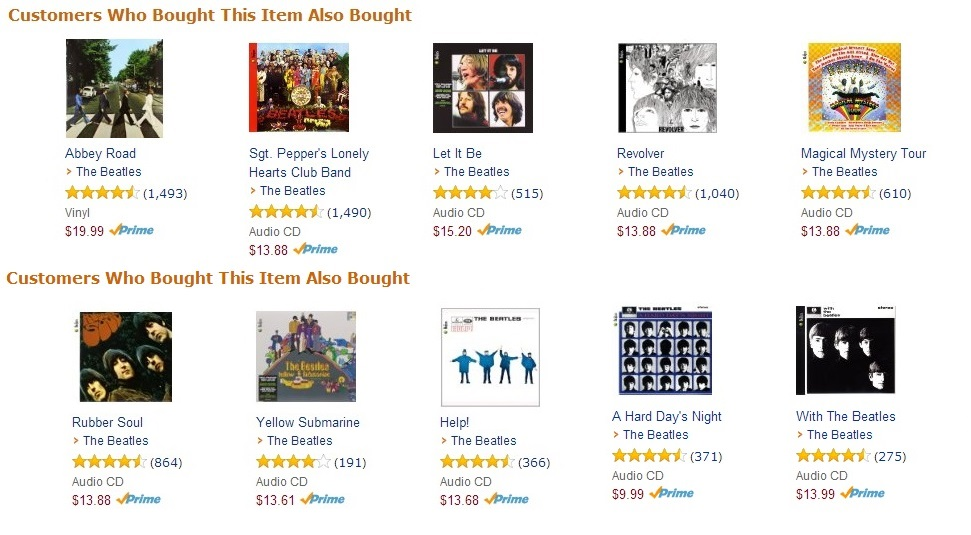
\includegraphics[scale=0.75]{beatles10.jpg}}
	\end{center}
	\caption{�lbuns recomendados pelo site Amazon.com ao pesquisar pelo White Album, dos Beatles. Os 10 primeiros s�o outros �lbuns dos Beatles. Busca realizada em Julho de 2014.}
	\label{fig:beatles}
\end{figure}


Relacionado com essa novidade em sistemas de recomenda��o, Vargas et al. \cite{vargas:2011} prop�em um modelo que relaciona usu�rios, itens e novidade. Existe uma diferen�a entre a descoberta (o usu�rio conhece um item, que deixa de ser novidade), a relev�ncia (item de interesse do usu�rio) e a escolha (quando o usu�rio seleciona um item relevante). Al�m disso, eles apontam que em geral as solu��es envolvendo novidades de itens s�o apresentadas em dois modelos: o modelo baseado em popularidade e o baseado na similaridade de itens previamente expostos. Este tipo de vis�o da novidade como dois modelos tamb�m � corroborado por Beloggin et. al \cite{Bellogin:2010}.

O modelo baseado em popularidade define que a popularidade do item est� relacionada � sua descoberta pelas pessoas. Quanto menos popular um item, menos ele foi descoberto pelas pessoas, possuindo uma maior probabilidade de ser novidade para a maioria das mesmas \cite{Celma:2008}.  V�rios trabalhos utilizam m�tricas relacionadas com a popularidade para detectar o quanto os algoritmos estudados exp�em novidades \cite{Celma:2008,Ziegler:2005,vargas:2011,Bellogin:2010,Zhang:2012}.

O modelo baseado em similaridade define que h� uma maior probabilidade de um item ser novidade para um usu�rio se este n�o for similar a outros itens descobertos e escolhidos pelo mesmo. Boa parte das abordagens baseadas neste tipo de modelo agrupam os itens em classes, como uma taxonomia, onde os itens s�o agrupados / rotulados nas classes a partir da similaridade dos mesmos. Assim, s�o recomendados para o usu�rio itens de classes que n�o s�o similares a classes anteriormente escolhidas pelo usu�rio \cite{Nakatsuji:2010,Ziegler:2005,Zhang:2012}.

%%%%%%%%%%%%%%%%%%%%%%%%%%%%%%%%%%%%%%%%%%%%%%%%%%%%%%%%%%%%%%%%%%%%%%%%%%%%%%%%%%%%%%%%%%%%%%%%%%%%%%%%%%%%%%%%%%%%%%%%%%%%%%%%%%%%%%%%%%%%%%%
\section{Grupos de pessoas baseados no comportamento}
Outro tema estudado no �mbito de novidades � a exist�ncia de diferentes grupos com diferentes prefer�ncias para novidades. Por exemplo, Munson e Resnick \cite{Munson:2010} descobriram, em um conjunto de usu�rios online, subgrupos baseados nas prefer�ncias por novas opini�es: apreciadores de diversidade, aversos a desafios e buscadores de apoio. Os apreciadores de diversidade s�o usu�rios que se interessam tanto por opini�es similares a suas quanto desafiadoras. Eles n�o se satisfazem com apenas opini�es similares. J� os aversos a desafios se satisfazem mais com opini�es semelhantes, diminuindo a satisfa��o se lerem opini�es desafiadoras. J� os buscadores de apoio se satisfazem com um certo n�mero de opini�es semelhantes, que suportam seu ponto de vista, sendo indiferentes a demais opini�es conflitantes. Este resultado mostra que diferentes pessoas possuem diferentes comportamentos frente a novidades (no estudo, novas opini�es).

Sobre a exist�ncia de diferentes grupos de pessoas no �mbito musical, Jennings \cite{Jennings} sumariza quatro grupos de pessoas baseados no grau de interesse por m�sica: os eruditos, entusiastas, casuais e indiferentes. Os eruditos s�o pessoas onde a m�sica � parte principal das suas vidas, possuindo conhecimento musical extensivo; os estusiastas s�o pessoas que consideram m�sica um aspecto muito importante, mas balanceam o interesse com outros temas; os casuais gostam de m�sica mas possuem consideram outros assuntos bem mais importantes e os indiferentes n�o se interessam por m�sica.

J� Arhippainen \& Hickey \cite{Arhippainen2011} conduziram uma pesquisa qualitativa e identificaram cerca de 14 grupos de ouvintes baseados em como eles escutam e usam m�sica no seu dia a dia. Dentre os 14 grupos, podemos destacar os Ouvintes Indie, que buscam constantemente novas m�sicas, Ouvintes do Mainstream, que escutam tudo que est� na m�dia e Ouvintes Passivos, que geralmente escutam o que outras pessoas est�o escutando.

\section{Nossas contribui��es}
Apesar de trabalhos passados utilizarem conceitos de novidade, tanto de itens musicais quanto de itens no geral, n�o foram encontrados estudos que relacionem diferentes aspectos das novidades com a relev�ncia das mesmas para os usu�rios. Como apontado na Se��o \ref{sec:nov_siscomp}, a novidade pode ser modelada em no m�nimo dois aspectos. Al�m disso, O' Celma \cite{Celma:2008} comenta que � importante sabermos a relev�ncia de novidades para os usu�rios, em um estudo "`centrado no usu�rio"', para que tenhamos um conhecimento mais completo do seu comportamento. Enquanto algumas abordagens para novidade fazem estudos "`centradas nos itens"', preocupadas principalmente nas caracter�sticas dos itens (como a popularidade).

Assim, n�s unimos os aspectos formalizados por Vagas e corroborados em v�rios estudos com a ideia de relev�ncia (estudo centrado no usu�rio), que O' Celma \cite{Celma:2008} corrobora a import�ncia. Com essa jun��o de conceitos podemos responder que aspectos das novidades s�o relevantes para ouvintes e consumidores musicais.

Al�m disso, outro resultado do nosso trabalho segue a linha de trabalhos sobre grupo de pessoas baseado no comportamento \cite{Munson:2010;Jennings;Arhippainen2011}. Descobrimos diferentes grupos de ouvintes baseados nas prefer�ncias dos mesmos pelos aspectos das novidades. Mesmo em contextos diferentes do trabalho de Munson\cite{Munson:2010} (opini�es e m�sica), podemos notar que novidade n�o pode ser tratado de forma �nica para todos os indiv�duos. Nossos resultados sugerem que h� uma necessidade de tratamento espec�fico para cada grupo, em um sistema computacional como sistema de recomenda��o, por exemplo. O'Celma \cite{CelmaBook:2010} refor�a este tipo de tratamento espec�fico para cada grupo.

Por fim, descobrimos que as prefer�ncias dos ouvintes frente aos aspectos dos artistas com novidade s�o diferentes das prefer�ncias frente aos aspectos dos artistas conhecidos. Isso sugere que a novidade no �mbito musical seja estudada especificamente, n�o podendo generalizar do que o ouvinte j� conhece.

\chapter{Conceitos e Modelos} \label{cap:aspectos_novidade}

Este cap�tulo define quais conceitos e modelos foram utilizados na pesquisa. Para a constru��o dos experimentos, primeiro foi definido o conceito de novidade que ir�amos trabalhar junto com o das suas caracter�sticas. Foi importante esta defini��o inicial pois os termos utilizados na pesquisa (novidade, familiaridade, popularidade, relev�ncia) s�o termos gerais, que podem possuir mais de um significado, n�o tendo um consenso da literatura. 

\section{Tipos dos itens estudados}
	
	Primeiro foi definido o que seria uma novidade, ou um item com novidade, e consequentemente um item conhecido.

	\subsection {Item com novidade / Novidade}
	
	Novidade � o conceito central deste trabalho. Um item com novidade � um item que n�o foi acessado pela pessoa anteriormente. No �mbito musical, itens podem ser m�sicas, artistas e �lbuns, e as pessoas que escutam esses itens s�o ouvintes. Mais especificamente, tratamos as novidades como artistas que n�o foram escutados anteriormente pelo ouvinte. Por exemplo, se em algum momento o ouvinte Jo�o escutou o artista Eminem pela primeira vez, Eminem deixou de ser uma novidade para ser um artista conhecido. Antes desse momento ele era considerado uma novidade para Jo�o.
	
	\subsection {Item conhecido}
	
	Um item conhecido � o oposto da novidade. Assim, � um item que j� foi acessado anteriormente pela pessoa. No nosso trabalho, um artista conhecido � um artista que j� foi escutado anteriormente pelo ouvinte. No Cap�tulo \ref{cap:comparacao} � mostrado o resultado da compara��o entre as prefer�ncias dos ouvintes pelas caracter�sticas dos artistas com novidade e as prefer�ncias do mesmo pelas caracter�sticas dos artistas conhecidos.

%%%%%%%%%%%%%%%%%%%%%%%%%%%%%%%%%%%%%%%%%%%%%%%%%%%%%%%%%%%%%%%%%%%%%%%%%%%%%%%%%%%%%%%%%%%%%%%%%%%%%%%%%%%%
\section{Caracter�sticas de um item}
	Para calcular a familiaridade de um artista para um ouvinte, foi necess�rio definir caracter�sticas do artista e do perfil musical do ouvinte, j� que a familiaridade est� relacionada com a similaridade do artista para o perfil do ouvinte. Neste contexto surge os conceitos de descritores e descri��o.

	\subsection{Descritores}
	 Um descritor � um um s�mbolo que descreve / caracteriza um item. No �mbito musical, descritores s�o termos que podem caracterizar m�sicas, artistas, �lbuns, perfis musicais de ouvintes, etc. Estes descritores podem representar g�nero musical (pop, forr�), localiza��o (latina, brasileira, brit�nica), humor (animada, depressiva), entre outros.

	\subsection{Descri��es} \label{subsec:descricoes}
	Um item pode ser caracterizado por mais de um descritor, e estes descritores caracterizam-no em menor ou maior grau. Tomemos como exemplo o artista Michael Jackson. Ele pode ser descrito pelos termos Pop, Dance e Soul. Destes termos, Pop o carateriza em um grau maior que Soul. Desta maneira, para uma carateriza��o completa dos itens, � necess�rio representar este conjunto de descritores. Para isso usamos o termo descri��o.
	Sejam $I$ o conjunto de itens, $D$ o conjunto de descritores e $g:I\times D\rightarrow \mathbb{R}$ a fun��o que denote o grau que o descritor $d\in D$ caracteriza o item $i\in I$. Assim, a descri��o $\theta_{i}$ de um item $i\in I$ � definida pela Equa��o \ref{eq:descricao}:

	\begin{equation}
	\theta_{i} = \{ (d_1 , g(i,d_1) ), \ldots, (d_{|\theta|} , g(i,d_{|\theta|}) ) \} \label{eq:descricao}
	\end{equation}

	Ou seja, � um conjunto de descritores junto com o grau que cada descritor caracteriza o item. Por exemplo, \{(pop, 0,7), (dance, 0,5), (soul, 0,5)\} pode ser considerada uma descri��o do artista Michael Jackson.
%%%%%%%%%%%%%%%%%%%%%%%%%%%%%%%%%%%%%%%%%%%%%%%%%%%%%%%%%%%%%%%%%%%%%%%%%%%%%%%%%%%%%%%%%%%%%%%%%%%%%%%%%%%%
\section{Representa��es do hist�rico musical}

\subsection{Artista}\label{subsec:modelo_artista}
Na nossa pesquisa, os itens com novidade e os itens conhecidos s�o artistas. Para calcular as m�tricas que foram utilizadas na pesquisa, definimos um modelo para as caracter�sticas dos artistas. Este modelo do artista possui uma descri��o e uma popularidade, que representa o quanto de pessoas no mundo conhecem este artista. Formalmente, sejam $A$ o conjunto de artistas, $\Theta$ o conjunto de descri��es, $\theta_{a} \in \Theta$ a descri��o do arista $a \in A$ e $p$ a popularidade do artista $a$, o modelo $w$ que caracteriza $a$ pode ser representado pela Equa��o \ref{eq:modelo_artista}:

	\begin{equation}
		w := (\theta_{a},p) \label{eq:modelo_artista}
	\end{equation}

\subsection{Perfil} \label{sec:perfil}

Um perfil de um usu�rio � um modelo que representa caracter�sticas de um determinado usu�rio sobre determinado tema. Assim, o perfil musical de um ouvinte � uma representa��o das m�sicas ou artistas que ele tipicamente escuta. A necessidade de uma representa��o do perfil musical do ouvinte surgiu primeiramente para calcular a familiaridade de um artista para o ouvinte. Al�m disso, utilizamos o perfil para extrair a ecleticidade do ouvinte e para gerar uma representa��o visual do que foi escutado pelo ouvinte

Uma forma de representa��o intuitiva do perfil de uma pessoa seria o conjunto de g�neros musicais de artistas que essa pessoa escuta/escutou. Tipicamente, ao perguntar a ouvintes qual seu perfil musical, respostas como estas surgem: "Geralmente escuto artistas de Rock", "Escuto mais bandas de Forr� e Pagode". � como se eles abstra�ssem os artistas, os agrupando baseado em seus g�neros musicais. Uma representa��o formal desse conceito se adequaria � nossa necessidade, pois g�neros musicais, como Forr�, Pagode e Rock, s�o considerados  descritores musicais. Dessa maneira seria poss�vel calcular a similaridade entre os descritores de um artista com os descritores do perfil musical do ouvinte.

Assim, o perfil musical de um pessoa � formado por um conjunto de pares (descri��o, relev�ncia) que descreve, para um dado per�odo, as caracter�sticas dos artistas escutados por essa pessoa e a frequ�ncia com que artistas com diferentes caracter�sticas foram escutados. Por exemplo, uma pessoa pode ter um perfil composto por \{(rock, brit�nico; 0,2 ), (rock, brasil; 0,15), (rock, eletr�nico; 0,1), ...\}, ou seja, ter escutados artistas de rock brit�nico representando 20\% do seu hist�rico musical, artistas de rock brasileiro representando cerca de 15\% do seu hist�rico e artistas de rock misturado com eletr�nico, representando 10\% do seu hist�rico. Formalmente, sejam $P_{\theta}$ o conjunto de descri��es do perfil $P$, $\theta_{i} \in P_{\theta}$ uma descri��o com relev�ncia $r_{i}$. O perfil $P$ de um ouvinte � formado por:

\begin{equation}
	\text{P} = \{(\theta_{i} , r_{i}) \}\label{eq:descricao}
\end{equation}

\subsubsection{Constru��o do Perfil}
Uma possibilidade para a constru��o do perfil � agrupar os artistas de acordo com a semelhan�a em suas descri��es e ent�o extrair uma descri��o que represente cada grupo de artista. Para realizar esse agrupamento, foi utilizado um algoritmo de agrupamento hier�rquico aglomerativo \cite{hastie}. Este tipo de algoritmo inicializa cada elemento (em nosso caso cada descri��o de cada artista) em um grupo, e a cada passo, ele une os dois grupos mais pr�ximos (similares). Desta maneira, foi necess�rio definir uma medida de dist�ncia, ou dissimilaridade, entre os grupos. 

Na maior parte dos m�todos utilizados no agrupamento hier�rquico aglomerativo, a medida de dist�ncia entre grupos pode ser gerada a partir de uma m�trica de dist�ncia entre os pares de elementos e um crit�rio de uni�o que especifica quais grupos unir em cada passo, em fun��o desta dist�ncia.  Ent�o, foi definido como m�trica de dist�ncia entre pares de descri��es dos artistas o complemento da similaridade do cosseno entre os vetores de descri��es dos artistas e como crit�rio de  uni�o (\textit{linkage criterion}) o agrupamento de uni�o pela m�dia (o \textit{average linkage clustering}).

A similaridade do cosseno entre as descri��es de dois artistas � definida pela Equa��o ~\ref{eq:cosine}. Como o algoritmo aglomerativo hier�rquico requer uma medida de dist�ncia, e n�o de similaridade, foi calculado o complemento da similaridade do cosseno (Equa��o \ref{eq:distancia}).

\begin{equation}
\text{cos}(\vec{\theta},\vec{\theta}'):=
      \frac{\langle \vec{\theta},\vec{\theta}' \rangle}{\|\vec{\theta}\| \|\vec{\theta}'\|}  \label{eq:cosine}
\end{equation}

\begin{equation}
\text{dis}(\vec{\theta},\vec{\theta}'):= 1 - \text{cos}(\vec{\theta},\vec{\theta}') \label{eq:distancia}
\end{equation}


 O \textit{average linkage clustering} \cite{hastie} � um m�todo de uni�o de grupos baseado na m�dia das dist�ncias entre cada par de elementos de cada grupo. A dist�ncia entre dois grupos � definida pela Equa��o ~\ref{eq:averageLinkage}. Sejam $X$ e $Y$ grupos, onde $x\in X$ a descri��o de um artista do grupo $X$ e $y \in Y$ a descri��o de um artista do grupo $Y$. A dist�ncia $d(X,Y)$ entre os grupos $X$ e $Y$ � definida pela m�dia das dist�ncias de todos os pares $x\in X$ e $y \in Y$ (Equa��o \ref{eq:averageLinkage}).
 
  \begin{equation}
\text{d}(X,Y):= \frac{1}  {\left| X \right| \left| Y \right|}\sum\limits_{x\in X}\sum\limits_{y\in Y} dis(x,y) \label{eq:averageLinkage}
\end{equation}

Ap�s a defini��o da dist�ncia entre grupos, o algoritmo de agrupamento foi aplicado para os artistas de cada ouvinte separadamente. Como � um m�todo aglomerativo hier�rquico, o algoritmo inicia a descri��o de cada artista dentro de um grupo separado. Em cada etapa os grupos mais pr�ximos v�o sendo aglutinados, at� chegar em 1 grupo com todos os artistas. � necess�ria uma condi��o de parada para selecionar o n�mero de grupos de um ouvinte adequado. Esta condi��o de parada vai ser comentada no Cap�tulo \ref{cap:dados}.

Assim, com o os grupos de artistas definidos, pode-se extrair o conjunto de pares (descri��o, relev�ncia) que representa o perfil. Para cada grupo de artistas, o centr�ide das descri��es dos artistas representa a descri��o daquele grupo, e a propor��o de todas as execu��es de m�sicas dos artistas deste grupo escutadas pelo ouvinte � a relev�ncia deste grupo no perfil do ouvinte. Quanto mais vezes os artistas do grupo $i$ foram escutados, mais influentes as descri��es deste grupo s�o para o ouvinte.

% 	Formalmente, sejam $P := \{C_1, ..., C_n\}$ o perfil do ouvinte, formado pelos grupos de artistas $C_i$ e $I := \{1, ..., n\}$ o conjunto �ndice de $P$. Sejam $\vec{c_i}$ o centr�ide do grupo $C_i$ e $p_i$ a influ�ncia do grupo  $C_i$ no perfil do ouvinte, definida como a propor��o de todas as execu��es de m�sicas pelo ouvinte que s�o as m�sicas cujos artistas est�o em $C_i$. 

% , o algoritmo foi interrompido no momento em que a dist�ncia m�nima entre 2 grupos fosse igual a 0,30. Este valor de 0,30 foi obtido empiricamente. Para tanto, foram selecionados alguns ouvintes com perfis musicais diferentes e foram analisados os grupos criados ao mudar este valor limite. O valor de 0,30 foi melhor valor encontrado na m�dia, onde -  no julgamento do autor desta disserta��o e de colegas do mesmo grupo de pesquisa - artistas similares estavam no mesmo grupo e artistas bastante diferentes estavam em grupos diferentes.


\subsection{Ecleticidade}  \label{subsec:eclet}

A ecleticidade representa o qu�o ecl�tico musicalmente um ouvinte � - o qu�o diferente s�o os grupos de artistas que ele escuta. Ou seja, um ouvinte com alta ecleticidade � um que escuta muitos estilos diferentes de m�sica.  Esta m�trica foi utilizada para conhecer melhor os h�bitos dos ouvintes e foi utilizada na gera��o dos grupos de ouvintes baseados nas prefer�ncias pelos aspectos das novidades comparadas com seus h�bitos musicais, descritos no Cap�tulo ~\ref{sec:grupos}. 
	
Inicialmente consideramos utilizar o n�mero de grupos do perfil do ouvinte como crit�rio de ecleticidade. Quanto mais grupos o ouvinte possu�sse no perfil, mais ecl�tico ele seria. Por�m, dois ouvintes podem possuir o mesmo n�mero de grupos mas um ouvinte pode possuir no perfil grupos mais similares (como um grupo de hip hop e outro de hip hop polon�s - Figura \ref{fig:cluster_pouca}) e outro possuir menos similares (como um grupo de pop e outro de industrial metal - Figura \ref{fig:cluster_muita}). 

\begin{figure}
\subfigure[Perfil com alta ecleticidade.]{
 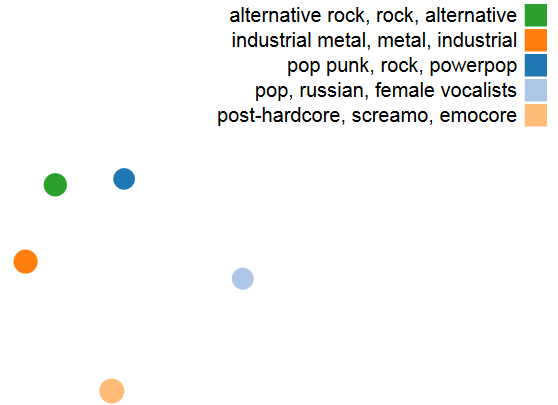
\includegraphics[height = 5cm]{figs/cluster_espalhado.png} \label{fig:cluster_muita}}
 \subfigure[Perfil com baixa ecleticidade]{
 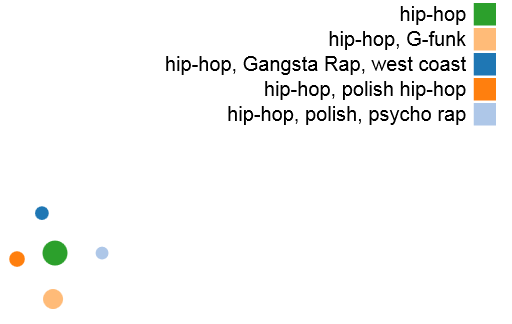
\includegraphics[height = 5cm]{figs/cluster_junto.png}  \label{fig:cluster_pouca}}
  \caption{Exemplos de dois perfis de ouvintes. Cada c�rculo representa um grupo de artistas e a dist�ncia entre os c�rculos � proporcional a similaridade entre os grupos. O tamanho de cada c�rculo � proporcional a quantidade de m�sicas dos artistas de cada grupo escutadas pelo ouvinte.}
  \label{fig:perfis}
\end{figure} 

Uma alternativa a essa abordagem seria contabilizar o quanto de diferen�a ou diversidade cada grupo adiciona ao perfil. Quanto mais diversidade houver nos grupos do perfil, mais ecl�tico o ouvinte �. Para isso, recorremos novamente a um algoritmo de agrupamento hier�rquico, por�m agora utilizando as descri��es do perfil como elementos a serem agrupados. A cada passo calculamos e armazenamos a dist�ncia entre os dois grupos que foram unidos. Por fim, definimos a ecleticidade como a soma de todas estas dist�ncias. Formalmente, sejam $P_{\theta}$ o conjunto de descri��es do perfil do ouvinte; $X^{(s)} := \{X^{(s)}_1, ...,X^{(s)}_{n}\}$ o conjunto de grupos no passo $s$ (\textit{step} � passo em ingl�s) do algoritmo hier�rquico, onde $X^{(1)} =  P_{\theta}$ e $X^{(j)}$, onde $j > 1$, s�o grupos do algoritmo hier�rquico criados a partir do conjunto inicial $X^{(1)}$. Seja $d(X^{(s)}_k,X^{(s)}_l)$ a dist�ncia entre os grupos $X^{(s)}_k$ e $X^{(s)}_l$. Ent�o, a ecleticidade do ouvinte com perfil $P$ � calculada na Equa��o ~\ref{eq:eclet}.

\begin{equation}
\text{e}(P)= 
      \sum_{s=1}^{|P| - 1} min_{k,l \in (1..|P-s+1|)} d(X^{(s)}_k,X^{(s)}_l)   \label{eq:eclet}
\end{equation}

A dist�ncia $d(X^{(s)}_k,X^{(s)}_l)$ entre os grupos do algoritmo hier�rquico foi calculada utilizando o  \textit{average linkage method} (Equa��o ~\ref{eq:averageLinkage}). Como o \textit{average linkage method} depende da dist�ncia entre cada par de elemento (onde cada elemento � uma descri��o), foi definido como dist�ncia entre dois grupos o complemento da similaridade do cosseno (Equa��o \ref{eq:distancia}) entre as descri��es.

\section {Aspectos}

Para caracterizar as novidades multidimensionalmente, utilizamos dois aspectos: a familiaridade e a popularidade. Esta se��o define estes dois aspectos.

\subsection{Familiaridade}	 \label{sec:familiaridade}
	Muitos trabalhos \cite{Nakatsuji:2010,Ziegler:2005,Zhang:2012} caracterizam uma novidade baseada na similaridade do item acessado pela pessoa em rela��o a outros itens acessados anteriormente pela mesma. Trazendo para o �mbito musical, rotulamos este tipo de caracter�stica como familiaridade. A familiaridade de um artista para um ouvinte reflete o quanto este ouvinte foi exposto a outros artistas que t�m descri��es semelhantes aos do artista escutado.
	
	Al�m da similaridade das descri��es, n�s levamos em conta o quanto estes artistas similares ao artista em quest�o foram escutados pelo ouvinte. Isso porque a familiaridade de um artista para um ouvinte � influenciado tamb�m pelo quanto este ouvinte escutou artistas similares ao artista em quest�o \cite{hargreaves:2002}. Por exemplo, se Maria tem h�bito de escutar muitos artistas pop e poucos artistas de rock, Britney Spears (cantora pop) � mais familiar a ela que Evanescence (banda de rock). Assim, a familiaridade est� relacionada com a similaridade entre a descri��o do artista e as descri��es do perfil do ouvinte junto com a influ�ncia desses artistas no perfil do ouvinte. 

	Formalmente, sejam $P$ o perfil do usu�rio, formado pelos pares de (descri��o $\theta_{i}$, relev�ncia $r_{i}$) e $\theta_{a}$ a descri��o do artista $a$. Assim, a familiaridade de $a$ para o perfil $P$ do ouvinte �: (Equa��o \ref{eq:simlaridade}).

	\begin{equation}
	\text{fam}(a,P)= 
	      max_{\theta_{i}, r_{i} \in P } cos(\vec{\theta_{a}},\vec{\theta_{i}}) \times r_{i}   \label{eq:simlaridade}
	\end{equation}

	\subsection {Popularidade}
	
	Outra caracter�stica bem relacionada com itens com novidade na literatura � a popularidade \cite{Celma:2008,Celma:20082,Ziegler:2005,vargas:2011,Bellogin:2010,Zhang:2012}. A rela��o feita � que, quanto menos popular um item, menos ele foi descoberto pelas pessoas, possuindo uma maior probabilidade de ser novidade para a maioria das mesmas \cite{Celma:2008}. Neste trabalho definimos a popularidade como sendo o quanto de pessoas j� escutaram o artista em quest�o. Por exemplo, Michael Jackson, artista que muitas pessoas de todo o mundo j� escutaram, � mais popular que Rapadura, um rapper brasileiro que foi escutado apenas por um nicho espec�fico de pessoas. A popularidade faz parte do modelo de um artista, descrito na Subse��o \ref{subsec:modelo_artista}.
	
	\section {Prefer�ncia dos itens pelos ouvintes}
	
	Com os aspectos familiaridade e popularidade, estudamos quais destas caracter�sticas das novidades s�o relevantes para o ouvinte. Em outras palavras, qual a prefer�ncia dos ouvintes por esses aspectos. Utilizamos dois conceitos de prefer�ncia:
	\begin{enumerate}
	
		\item Aten��o total
		
		� o quanto de aten��o que um ouvinte deu para o artista em um per�odo especificado. Para isso utilizamos a quantidade de m�sicas do artista que o ouvinte escutou no per�odo. Quanto mais m�sicas do artista, mais aten��o o ouvinte devotou ao artista.
		
		\item Per�odo de aten��o
		
		� o per�odo em que o ouvinte devotou de aten��o ao artista. No nosso trabalho, a unidade de tempo � uma semana. Assim, quanto mais semanas o ouvinte escutou alguma m�sica do artista em quest�o, maior o per�odo de aten��o do ouvinte.
	\end{enumerate}	


\chapter{Dados utilizados} \label{cap:dados}

Ap�s a descri��o das caracter�sticas das novidades (e dos artistas conhecidos) utilizadas no nosso estudo, esta se��o descreve os dados que foram utilizados na pesquisa. Podemos dividir os dados em 2 partes: a primeira � representada pelo hist�rico musical dos sujeitos a serem analisados e a segunda pelos metadados dos artistas escutados pelos sujeitos. Os sujeitos dos experimentos representam os ouvintes. O hist�rico musical foi utilizado para identificar os artistas com novidade, os artistas conhecidos e as prefer�ncias dos ouvintes por ambas. J� os metadados foram utilizados para identificar os aspectos dos artistas - a familiaridade e a popularidade. Os dados foram coletados da plataforma do Last.FM.

\section{Last.FM}

O Last.FM � uma rede social musical que tem como principal caracter�stica o \textit{Scrobbling} - um servi�o que permite registar o hist�rico de m�sicas escutadas pelos usu�rios. Al�m disso, o site fornece outros recursos como: servi�o de r�dio online, recomendador de novidades, tabelas com detalhes do hist�rico de execu��o do usu�rio, informa��es sobre artistas, turn�s e possibilidade de cria��o de f�runs.


O Last.FM fornece uma API \footnote{www.lastfm.com.br/api}(Application Programming Interface - conjunto de rotinas fornecidas por um software para que aplicativos acessem suas funcionalidades)  que permite o acesso a dados presentes no site. � poss�vel coletar informa��es dos usu�rios, hist�rico de escuta dos usu�rios e informa��es sobre m�sicas / �lbuns / artistas. Para nossos experimentos, n�s coletamos 2 tipos de dados: o primeiro consiste num conjunto de usu�rios junto com seu hist�rico de escuta e o segundo em metadados dos artistas escutados. Os usu�rios do Last.FM foram os sujeitos da pequisa, e como dito anteriormente, representam os ouvintes. 

	\section{Ouvinte}

Com o intuito de estudar os artistas escutados pelos ouvintes, foram coletados dados acerca de uma amostra de usu�rios do Last.FM. A amostragem que constituiu esse conjunto de usu�rios foi feita a partir do procedimento de \textit{SnowBall Sampling} \cite{goodman1961}, iniciada pelo perfil do autor e sendo expandida pela coleta dos vizinhos musicais. Vizinho musical � um conceito utilizado no Last.FM, onde duas pessoas s�o vizinhas se possu�rem gostos musicais parecidos. Foi coletado um conjunto de 100 mil usu�rios.

Ap�s a sele��o dos usu�rios, o pr�ximo passo foi coletar o hist�rico de escuta dos mesmos. Para identificar as novidades, o hist�rico do usu�rio foi dividido em per�odos, que ser�o detalhados a seguir.
 
	\subsection{Linha do Tempo}\label{sec:timeline}
	
	Os dados referentes ao hist�rico de cada sujeito foram coletados no per�odo entre a primeira vez que o usu�rio escutou alguma m�sica no Last.FM e Agosto de 2013. Este per�odo foi dividido em duas partes, como pode-se ver na Figura ~\ref{fig:timeline}: \textit{Hist�rico Inicial} do sujeito e o \textit{Per�odo de Experimento}. O Hist�rico Inicial contempla o per�odo desde a primeira m�sica que o sujeito escutou no Last.FM at� Agosto de 2012, enquanto o Per�odo de Experimento engloba o per�odo entre Agosto de 2012 e Agosto de 2013 (um ano no total). Al�m dessa divis�o, especificamos os seis primeiros meses do Per�odo de Experimento como \textit{Per�odo de Observa��o}.
	
	\begin{figure}[htbp]	
\begin{center}
		\fbox{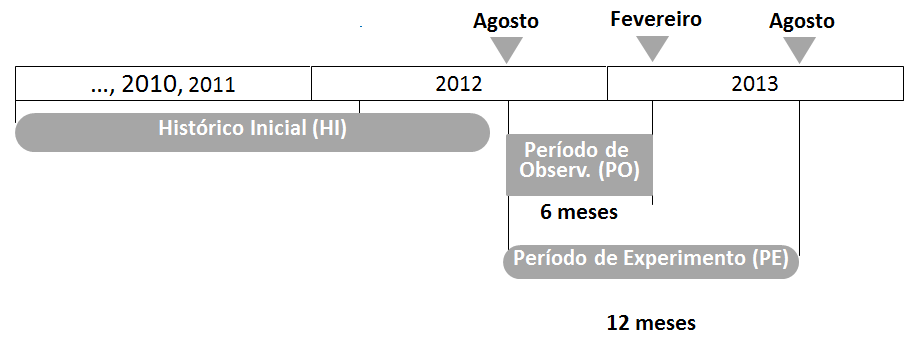
\includegraphics[scale=0.75]{timeline.png}}
	\end{center}
	\caption{Linha do tempo utilizada no trabalho}
	\label{fig:timeline}
\end{figure}


	Com esta divis�o, foram identificadas quais as novidades escutadas pelo usu�rio. Os artistas escutados pelo usu�rio no Per�odo de Observa��o que n�o foram escutados no Hist�rico Inicial s�o consideradas novidades. J� os artistas que foram previamente escutados no Hist�rico Inicial s�o considerados como artistas conhecidos. N�o consideramos o Per�odo de Experimento todo para evitar vi�s no c�lculo das caracter�sticas das novidades. Uma novidade a que um sujeito foi exposto no come�o do Per�odo de Experimento tem maior probabilidade de ser escutada mais vezes que uma novidade � qual o sujeito foi exposto no final do Per�odo de Experimento. Assim, identificamos como novidades os artistas escutados no Per�odo de Observa��o e levamos em conta as m�tricas referente a elas durante todo o Per�odo de Experimento (idem para os artistas conhecidos). Isso faz com que nossos dados tenham ao menos 6 meses de observa��o de cada novidade descoberta pelos sujeitos. 
	

	\subsection{Hist�rico do usu�rio}
	
	Do Hist�rico Total do ouvinte, coletamos todos os artistas que ele escutou desde a entrada do usu�rio no Last.FM at� Agosto de 2013, junto com o total de execu��es das m�sicas do artista. O m�todo da API utilizado foi \textit{getTopArtists}, que possibilta coletar os \textit{n} artistas mais escutados pelo ouvinte, onde este \textit{n} pode ser at� o n�mero total de artistas escutados por ele. Para o Per�odo de Experimento, fizemos dois tipos de coleta. A primeira, utilizando o \textit{getTopArtists} dos 12 meses, coletamos todos os artistas escutados, junto com o n�mero de execu��es das m�sicas de cada. O intuito dessa primeira coleta foi identificar os artistas do Hist�rico Inicial. A segunda parte consiste  nos artistas escutados em cada semana deste per�odo, junto com o n�mero de execu��es em cada semana. O m�todo da API do Last.FM utilizado foi o \textit{getWeeklyArtistChart}. Esta segunda coleta foi realizada com o intuito de obter,  al�m do n�mero de execu��es das m�sicas de cada artista, o n�mero de semanas em que o usu�rio escutou cada artista.
	
	Com os dados do Hist�rico Total e do Per�odo de Experimento conseguimos identificar o Hist�rico Inicial e as novidades. Os artistas do Hist�rico Inicial s�o os artistas que o ouvinte n�o escutou apenas no Per�odo de Experimento. Ou seja, artistas com n�mero de execu��es no Hist�rico Total do ouvinte maior que no Per�odo do Experimento. J� as novidades s�o os artistas com o mesmo n�mero de execu��es no Hist�rico Total e no Per�odo de Experimento.
		
	Ap�s a coleta e defini��o de cada per�odo, foi realizado uma filtragem nos dados, descrita a seguir.
	
	\subsection{Filtros}\label{sec:Filtros}
	
	Como o Last.FM � uma rede social formada por diferentes tipos de usu�rios com diferentes h�bitos musicais, julgamos necess�ria uma filtragem nos sujeitos, para selecionar os adequados aos prop�sitos dos experimentos. Abaixo est�o as caracter�sticas que os sujeitos precisavam ter para serem selecionados, junto com a maneira de filtragem utilizada.
	
\begin{enumerate}
	\item Possuir alta atividade de escuta no per�odo de Hist�rico Inicial.
	
	\textit{Filtro: Exclus�o de usu�rios que tenham escutado menos de 100 artistas no per�odo de Hist�rico Inicial.}
	\item Possuir alta atividade de escuta no Per�odo de Experimento.
	
	\textit{Filtro: Exclus�o de usu�rios que escutaram menos de 100 m�sicas por semana em pelo menos 1/4 das semanas do Per�odo de Experimento.}
	\item Serem expostos a um n�mero de novidades que permita a investiga��o de rela��es entre as caracter�sticas das novidades e as suas prefer�ncias.
	
		\textit{Filtro: Exclus�o de usu�rios que escutaram menos de 10 novidades.}
				
	\item Possuir n�mero realista de execu��es: foi detectado que alguns usu�rios possu�am um n�mero muito grande de execu��es musicais. Alguns, por exemplo, tiveram uma m�dia de mais de uma m�sica por minuto durante o per�odo de observa��o, o que na realidade � impratic�vel. Uma explica��o para esse fato seria a cria��o de rob�s que trocassem a m�sica assim que o sistema contabilizasse a execu��o da m�sica (dependendo da configura��o, o Last.FM pode considerar que a m�sica foi escutada se ela foi tocada por um certo tempo, como 30 segundos).
	
		\textit{Filtro: Exclus�o de usu�rios que tiveram uma m�dia de execu��es superior a 16 horas de execu��es por dia, no Per�odo de Experimento. Como as pessoas dormem em m�dia 8 horas por dia, um ouvinte que passe o dia todo, enquanto acordado, escutando m�sica, ele escutaria 16 horas de m�sica por dia. Suponto que uma m�sica tem em m�dia 4 minutos, foram exclu�dos os usu�rios que tiveram m�dia maior que 240 m�sicas por dia ($\frac{16hrs \times 60min}{4min / musica} = 240 musicas / dia$)}
	\item N�o utilizem majoritariamente a r�dio do Last.FM: um dos objetivos da pesquisa � identificar as prefer�ncias dos usu�rios. Assim, � importante que a maior parte dos artistas escutados pelo usu�rio sejam escolhidos por ele e n�o por uma r�dio.
	
	\textit{Filtro: Exclus�o de usu�rios que n�o escutaram nenhum artista mais de 15x na semana, em mais de 1/4 das semanas do per�odo de observa��o. 
	15 m�sicas � o n�mero m�dio de faixas que um �lbum cont�m. Desta maneira, se um usu�rio escutou mais de 15 m�sicas de um artista em uma semana, estamos supondo que ou o usu�rio escolheu escutar um �lbum do artista ou selecionou explicitamente 15 m�sicas do artista. Pela maneira como funciona a licen�a de direitos autorais para r�dios, � bastante improv�vel que mais de 15 m�sicas de um artista sejam executadas pela r�dio do Last.FM em uma semana. }
\end{enumerate}



O processo de filtragem resultou em uma amostra de 11.989 sujeitos. A Tabela \ref{tab:sumario} traz um sum�rio dos dados coletados.

\begin{table}[htpb]
\begin{center}
\begin{tabular}{|c|c|c|}
\hline
  & Artistas com novidade & Artistas conhecidos\\
\hline
Total & 389.853 & 1.202.869 \\
M�dia por ouvinte (desvio padr�o) & 32,5 (26,75) & 100,33 (60,03) \\
\hline
\end{tabular}
\end{center}
\caption{Sum�rio dos dados coletados.}
\label{tab:sumario}
\end{table}

 
	\section{Metadados dos Artistas}\label{sec:Artista}
Com o intuito de construir o modelo de artista descrito na Subse��o \ref{subsec:modelo_artista} e com isso calcular os aspectos das novidades, foram coletados dois tipos de metadados referentes aos artistas: as \textit{tags} que descrevem o artista (representando os descritores do artista) e a popularidade do artista no Last.FM. 

\textit{Tags} s�o palavras (ou conjunto de palavras), como \textit{rock}, \textit{rap} e \textit{pop}, associadas a um recurso, como m�sicas, �lbuns e artistas . No Last.FM os usu�rios podem marcar cada um dos recursos com alguma tag, caracterizando-as \textit{tags sociais}. Estas tags podem representar g�neros musicais (rock, samba), localiza��o (brasil, nordeste, germany, west coast), humor (sad, chill, happy), opini�o (love, favorite), refer�ncia pessoal (seen live, i own it), entre outros. Como as tags podem ser de v�rios tipos (n�o apenas g�nero musical), elas podem ser consideradas \textit{descritores} dos artistas.

Para cada artista foram coletadas as tags atribu�das a ele pelos usu�rios, junto com a popularidade de cada tag. Esta popularidade est� relacionada � quantidade de vezes que a tag foi atribu�da para o artista espec�fico, pelos usu�rios do Last.FM. A popularidade da tag fornecida pelo Last.FM � normalizada, onde a tag mais atribu�da possui valor igual a 100 e as outras tags possuem valores proporcionais, de acordo com a frequ�ncia de atribui��o de cada uma. Esta popularidade representa o grau de caracteriza��o do descritor para o artista, como discutido na Subse��o \ref{subsec:descricoes}. Formalmente, sejam $A$ o conjunto de artistas, $T$ o conjunto de tags e $h:A\times T\rightarrow \mathbb{R}$ uma fun��o que denote a frequ�ncia absoluta que uma tag $t\in T$ foi atribu�da a um artista $a\in A$. O valor normalizado da tag $t$, representado pela fun��o $f:A\times T\rightarrow \mathbb{R}$ � representado pela Equa��o ~\ref{eq:freqrel}.

\begin{equation}
  f(t,a) = \frac{h(t,a)}{max_{x\in T} h(x,a)} \times 100 \label{eq:freqrel}
\end{equation} 

A Tabela ~\ref{tab:tabelaTags} apresenta as 5 tags com maior valor do artista Michael Jackson. Pode-se ver que a tag \textit{pop} foi a mais atribu�da para Michael Jackson, possuindo valor 100. O m�todo utilizado da API do Last.fm foi o \textit{artist.gettoptags}.




\begin{table}[htpb]
\begin{center}
\begin{tabular}{|c|c|}
\hline
Tag & Valor  \\
\hline
pop & 100  \\
80s & 49 \\
dance & 40 \\
soul & 35 \\
funk & 32 \\
\hline
\end{tabular}
\end{center}
\caption{Tags do artista Michael Jackson, junto com o valor normalizado de cada uma.}
\label{tab:tabelaTags}
\end{table}


Como as tags s�o associadas pelos usu�rios do Last.FM, h� problemas relacionadas a esse processo \cite{lamere:2008}. Usu�rios podem atribuir tags que n�o condizem com a realidade, podem errar na escrita da tag, etc. Para utilizar tags que realmente descrevam o artista, foi realizado um processo de filtragem. De cada artista foram consideradas as tags populares at� um m�ximo de 4 tags, tendo cada uma popularidade m�nima de 30 (onde a tag mais atribu�da �quele artista possui valor de 100). Al�m disso, foram eliminadas manualmente as tags com conota��o pessoal, como \textit{seen live} (vi ao vivo) ou \textit{favorite} (favorito).

Sobre a popularidade do artista, foram coletados o n�mero de usu�rios do Last.FM que escutaram cada artista. A Tabela \ref{tab:tabelaPopularidade} mostra exemplos de popularidade de alguns artistas. O m�todo utilizado da API foi o \textit{artist.getinfo}.

\begin{table}[htpb]
\begin{center}
\begin{tabular}{|c|c|}
\hline
Artista & N�mero de ouvintes (popularidade)  \\
\hline
Michael Jackson & 2.998.428  \\
The Beatles & 3.177.625 \\
Red Hot Chili Peppers & 4.032.453 \\
Eminem & 3.756.890 \\
Chico Buarque & 314.584 \\
\hline
\end{tabular}
\end{center}
\caption{N�mero de ouvintes (popularidade) de alguns artistas no Last.FM}
\label{tab:tabelaPopularidade}
\end{table}

%%%%%%%%%%%%%%%%%%%%%%%%%%%%%%%%%%%%%%%%%%%%%%%%%%%%%%%%%%%%%%%%%%%%%%%%%%%%%%%%%%%%%%%%%%%%%%%%%%%%%%%%%
\section{Aplica��o dos dados nos modelos}
Esta Se��o remete os modelos discutidos no Cap�tulo \ref{cap:aspectos_novidade}, agora relacioando os modelos com os dados coletados.

\subsection{Perfil}

Como dito anteriormente, o perfil musical de um pessoa � formado por um conjunto de pares (descri��o, relev�ncia) que descrevem as caracter�sticas dos artistas escutados por essa pessoa e a frequ�ncia com que artistas com diferentes caracter�sticas foram escutados. Para a constru��o do perfil foram utilizados os artistas do hist�rico musical do sujeito que n�o foram consideradas novidades. Assim, as descri��es utilizadas s�o as tags dos artistas junto com a popularidade de cada tag para o artista.

O m�todo utilizado para construir o perfil foi algoritmo de agrupamento hier�rquico aplicado nas descri��es dos artistas. Como � um m�todo aglomerativo hier�rquico, o algoritmo inicia cada descri��o dos artistas dentro de um grupo separado. Em cada etapa os grupos mais pr�ximos v�o sendo aglutinados, at� chegar em 1 grupo com todos os artistas. Para selecionar o n�mero de grupos de um ouvinte, o algoritmo foi interrompido no momento em que a dist�ncia m�nima entre 2 grupos fosse igual a 0,30 (lembrando que foi utilizado o complemento da similaridade do cosseno entre os vetores de descri��es como c�lculo de dist�ncia. Os detalhes foram expostos na Subse��o \ref{sec:perfil}). Este valor de 0,30 foi obtido empiricamente. Para tanto, foram selecionados alguns ouvintes com perfis musicais diferentes e foram analisados os grupos criados ao mudar este valor limite. O valor de 0,30 foi melhor valor encontrado, onde -  no julgamento do autor desta disserta��o e de colegas do mesmo grupo de pesquisa - artistas similares estavam no mesmo grupo e artistas bastante diferentes estavam em grupos diferentes.

Os perfis obtidos tiveram m�dia de 33,28 pares de (descri��o , relev�ncia), onde cada par estava relacionado a pelo menos 2 artistas (foram exclu�dos os pares relacionados a apenas um artista, considerados outliers), e desvio padr�o de 20,3. A Figura \ref{fig:ecdf_clusters} representa o gr�fico de distribui��o acumulada do n�mero de pares encontrados nos perfis dos sujeitos selecionados em nosso experimento. A Figura \ref{fig:perfis} representa dois exemplos de perfis.
		\begin{figure}[htbp]	
\begin{center}
		\fbox{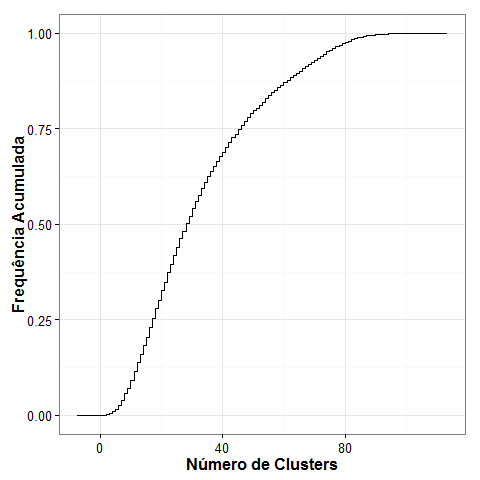
\includegraphics[scale=0.45]{ecdf_clusters.png}}
	\end{center}
	\caption{Distribui��o acumulada do n�mero de grupos}
	\label{fig:ecdf_clusters}
\end{figure}


%%%%%%%%%%%%%%%%%%%%%%%%%%%%%%%%%%%%%%%%%%%%%%%%%%%%%%%%%%%%%%%%%%%%%%%%%%%%%%%%%%%%

\subsection{Ecleticidade} \label{subsec:eclet}

Com as descri��es dos perfis dos ouvintes calculadas foi poss�vel calcular a ecleticidade de cada ouvinte. A Figura \ref{fig:perfis} compara dois perfis de ouvintes com ecleticidades bastante diferentes. A Figura \ref{fig:cluster_muita} � o perfil de um ouvinte mais ecl�tico que o ouvinte da Figura \ref{fig:cluster_pouca}.

%%%%%%%%%%%%%%%%%%%%%%%%%%%%%%%%%%%%%%%%%%%%%%%%%%%%%%%%%%%%%%%%%%%%%%%%%%%%%%%%%%%%

\subsection{Familiaridade} 


\begin{figure}
\subfigure[Artistas com novidade]{
 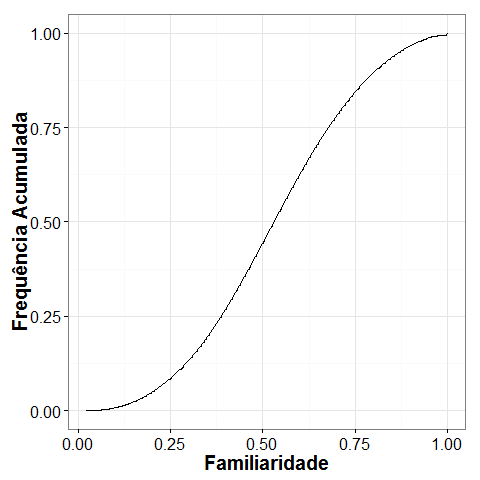
\includegraphics[width=.45\columnwidth]{figs/ecdf_n_fam.png} \label{fig:ecdf_fam_new}}
 \subfigure[Artistas conhecidos]{
 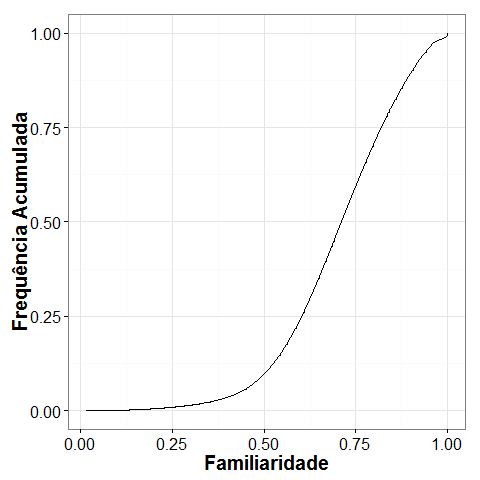
\includegraphics[width=.45\columnwidth]{figs/ecdf_old_fam.png}  \label{fig:ecdf_fam_old}}
  \caption{Frequ�ncia acumulada da familiaridade dos artistas para os ouvintes.}
  \label{fig:ecdf_fam}
\end{figure} 



Com o perfil dos ouvintes calculados foi poss�vel calcular a familiaridade dos artistas para os ouvintes. A Figura \ref{fig:ecdf_fam} representa gr�ficos da distribui��o acumulada da familiaridade dos artistas para os ouvintes. Podemos observar que os valores da familiaridade para os artistas com novidade (Figura \ref{fig:ecdf_fam_new}) s�o em geral menores que os valores para os artistas conhecidos (Figura \ref{fig:ecdf_fam_old}).

\subsection{Popularidade}
Para calcular a popularidade, utilizamos o logaritmo na base 10 do n�mero de ouvintes do artista no Last.FM. O logaritmo foi utilizado pois a distribui��o da popularidade dos artistas � enviesada (\ref{fig:listeners_lastfm}).

	
\begin{figure*}[htp]
  \centering
  \subfigure[N�mero de ouvintes dos artistas]{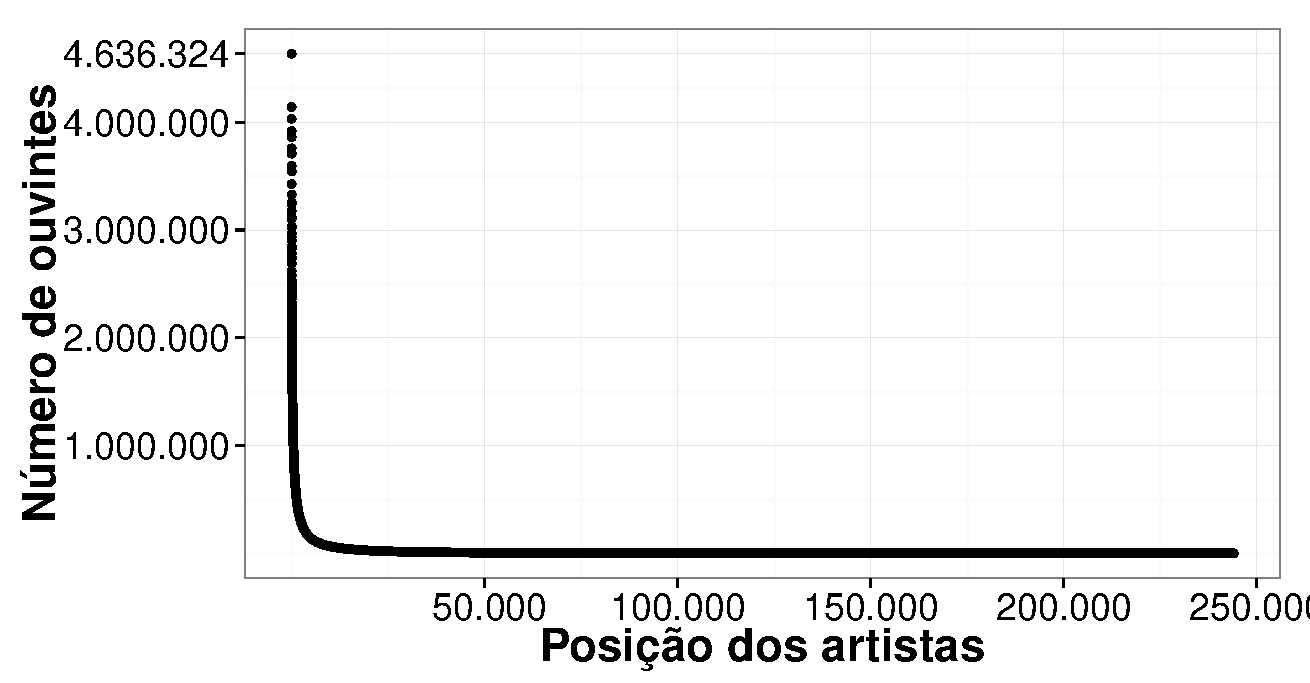
\includegraphics[scale=0.45]{figs/listeners.pdf}\label{fig:listeners}}\quad
  \subfigure[N�mero de ouvintes dos artistas (log linear)]{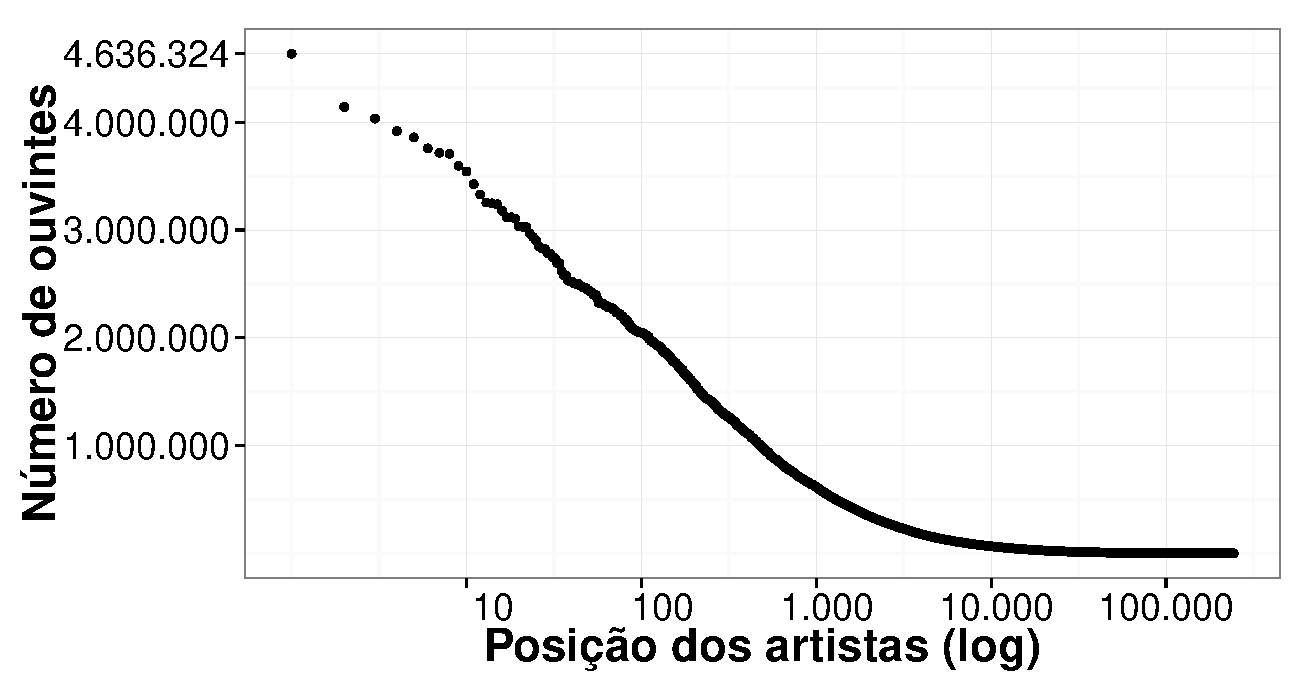
\includegraphics[scale=0.45]{figs/listeners_log.pdf} \label{fig:listeners_log} }
  \caption{N�mero de ouvintes dos artistas do Last.fm}
  \label{fig:listeners_lastfm}
\end{figure*}

A Figura \ref{fig:ecdf_pop} representa gr�ficos da distribui��o acumulada da popularidade dos artistas escutados pelos ouvintes. Podemos observar que os valores da popularidade dos artistas com novidade (Figura \ref{fig:ecdf_pop_new}) s�o em geral um pouco menores que os valores para os artistas conhecidos (Figura \ref{fig:ecdf_pop_old}).

\begin{figure}
\subfigure[Artistas com novidade]{
 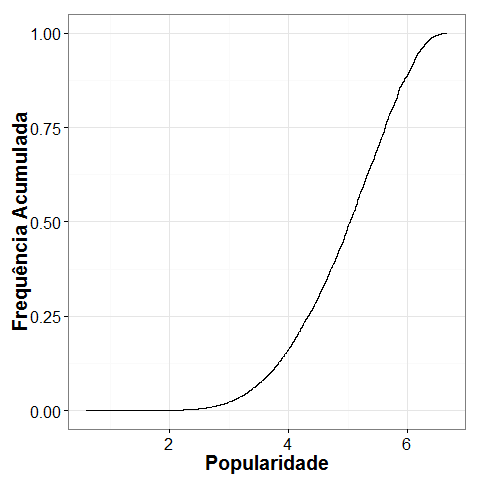
\includegraphics[width=.45\columnwidth]{figs/ecdf_n_pop.png} \label{fig:ecdf_pop_new}}
 \subfigure[Artistas conhecidos]{
 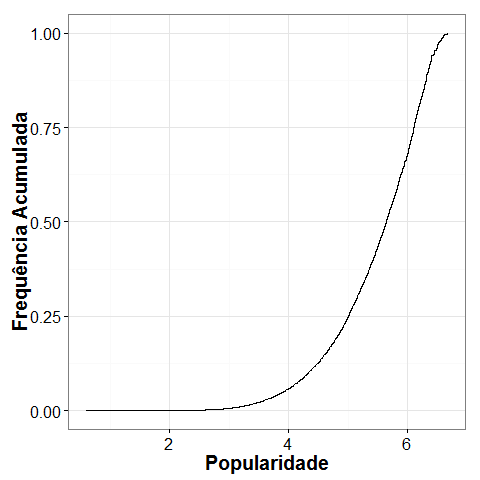
\includegraphics[width=.45\columnwidth]{figs/ecdf_old_pop.png}  \label{fig:ecdf_pop_old}}
  \caption{Frequ�ncia acumulada da popularidade dos artistas escutados pelos ouvintes (j� com valor transformado pelo log na base 10).}
  \label{fig:ecdf_pop}
\end{figure} 

\subsection{Prefer�ncias}
	Para mensurar o quanto o ouvinte gostou da novidade, foram utilizados duas m�tricas: a aten��o total e o per�odo de aten��o.  Como novidades podem ser descobertas em todo o Per�odo de Experimento, alguns destes artistas possuem uma janela de tempo no experimento menor (artistas escutadas no final do Per�odo de Experimento). Para contornar esse problema, utilizamos duas solu��es. Primeiro, utilizamos como denominador no c�lculo das m�tricas o n�mero de semanas da Janela de Tempo de exposi��o � novidade, que vai da primeira semana que foi escutada a novidade at� o fim do Per�odo de Experimento. Segundo, como mencionado na Se��o ~\ref{sec:timeline}, apenas as novidades descobertas no Per�odo de Observa��o foram consideradas na an�lise, mas todo o Per�odo de Experimento foi utilizado para c�lculo das m�tricas. Isso d� a cada novidade um m�nimo de 6 meses de coleta de dados, que limita um poss�vel vi�s para Janelas de Tempo pequenas.
	
	A aten��o total representa a aten��o que o ouvinte deu para o artista no Per�odo de Experimento. A aten��o total do ouvinte para o artista � representada pelo total de n�mero de execu��es de m�sicas do artista que ele escutou no Per�odo de Experimento, dividido pelo n�mero de semanas de sua Janela de Tempo. 
		
	J� o per�odo de aten��o o tempo que o ouvinte deu aten��o ao artista. Assim, � o n�mero de semanas que o ouvinte escutou o artista dividido pelo n�mero de semanas de sua Janela de Tempo.
	


%	\chapter{Modelos} \label{cap:modelos}
	
	Ap�s a coleta e filtragem dos dados, utilizamos 3 conceitos para representar as entidades envolvidas no estudo: modelo de perfil do ouvinte, caracter�sticas das novidades e m�tricas de relev�ncia. Primeiro, foi construindo o modelo do perfil do ouvinte, com o intuito de: gerar uma representa��o visual do que foi escutado pelo ouvinte; viabilizar o c�lculo da familiaridade de um artista para um ouvinte; e gerar uma m�trica de ecleticidade. Segundo, foram modeladas as caracter�sticas da novidade a serem utilizadas nos experimentos - familiaridade e popularidade. Por fim, foram modeladas duas m�tricas que refletem a prefer�ncia do ouvinte para um artista, ou a relev�ncia deste artista para o ouvinte, durante um per�odo de tempo - a aten��o total e o per�odo de aten��o.
 
	\section{Perfil musical do ouvinte}\label{sec:perfil}
 

Os artistas do hist�rico musical utilizados para a constru��o do perfil foram os que n�o s�o novidades e que possu�ssem n�mero de execu��o no hist�rico do usu�rio maior que a m�dia do n�mero de execu��es total dos artistas do hist�rico do usu�rio. Desta maneira utilizamos apenas os artistas mais representativos do perfil do ouvinte.

 

Os perfis obtidos tiveram m�dia de 33,28 grupos (onde cada grupo possui pelo menos 2 artistas) e desvio padr�o de 20,3. A Figura \ref{fig:ecdf_clusters} representa o gr�fico de distribui��o acumulada do n�mero de grupos de artistas encontrados nos perfis dos sujeitos selecionados em nosso experimento. A Figura \ref{fig:perfis} representa dois exemplos de perfis.
		\begin{figure}[htbp]	
\begin{center}
		\fbox{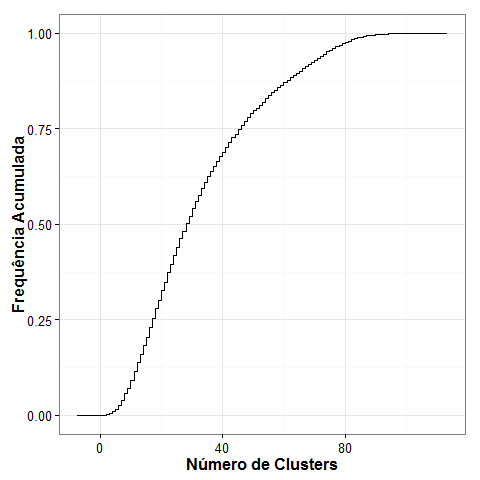
\includegraphics[scale=0.45]{ecdf_clusters.png}}
	\end{center}
	\caption{Distribui��o acumulada do n�mero de grupos}
	\label{fig:ecdf_clusters}
\end{figure}

A cria��o do perfil, al�m de auxiliar na visualiza��o do gosto musical do usu�rio, evidenciado nas Figuras \ref{fig:perfis}, e do c�lculo da familiaridade (Se��o ~\ref{sec:familiaridade}), faz parte do c�lculo da ecleticidade.	

\begin{figure}
\subfigure[Perfil com alta ecleticidade.]{
 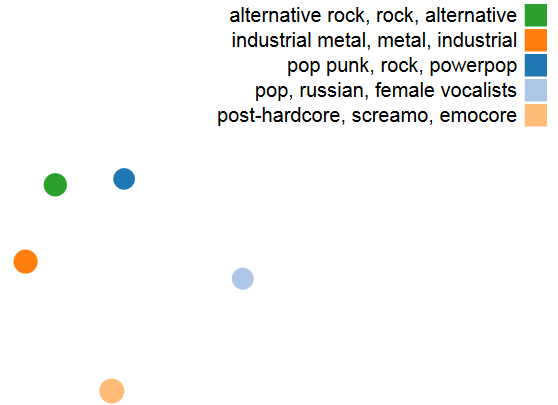
\includegraphics[height = 5cm]{figs/cluster_espalhado.png} \label{fig:cluster_muita}}
 \subfigure[Perfil com baixa ecleticidade]{
 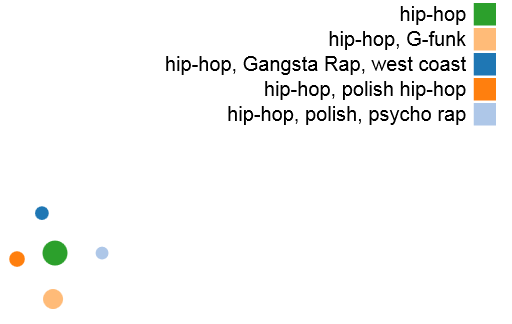
\includegraphics[height = 5cm]{figs/cluster_junto.png}  \label{fig:cluster_pouca}}
  \caption{Exemplos de dois perfis de ouvintes. Cada c�rculo representa um grupo de artistas e a dist�ncia entre os c�rculos � proporcional a similaridade entre os grupos. O tamanho de cada c�rculo � proporcional a quantidade de m�sicas dos artistas de cada grupo escutadas pelo ouvinte.}
  \label{fig:perfis}
\end{figure} 


	\subsection{Ecleticidade} \label{subsec:eclet}


A Figura \ref{fig:perfis} compara dois perfis de ouvintes com ecleticidades bastante diferentes. A Figura \ref{fig:cluster_muita} � o perfil de um ouvinte mais ecl�tico que o ouvinte da Figura \ref{fig:cluster_pouca}. Nota-se a diferen�a de ecleticidade pela dist�ncia entre os c�rculos. Enquanto na Figura \ref{fig:cluster_muita} os c�rculos est�o mais espassados, na Figura \ref{fig:cluster_pouca} os c�rculos est�o mais coesos.

	\section{Caracter�sticas das novidades}  
	

	\subsection{Familiaridade} 


\begin{figure}
\subfigure[Artistas com novidade]{
 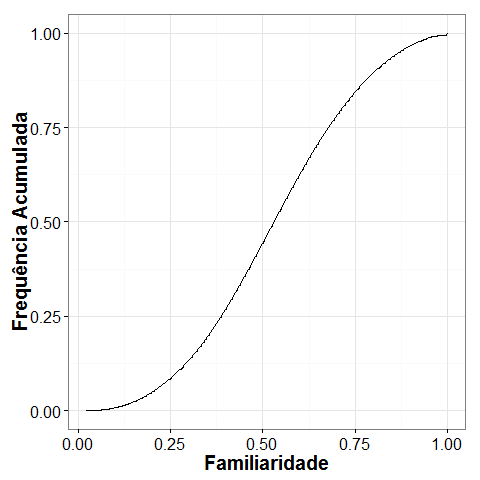
\includegraphics[width=.45\columnwidth]{figs/ecdf_n_fam.png} \label{fig:ecdf_fam_new}}
 \subfigure[Artistas conhecidos]{
 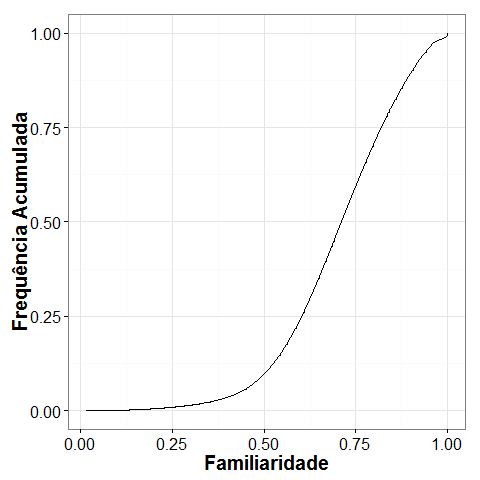
\includegraphics[width=.45\columnwidth]{figs/ecdf_old_fam.png}  \label{fig:ecdf_fam_old}}
  \caption{Frequ�ncia acumulada da familiaridade dos artistas para os ouvintes.}
  \label{fig:ecdf_fam}
\end{figure} 



A Figura \ref{fig:ecdf_fam} representa gr�ficos da distribui��o acumulada da familiaridade dos artistas para os ouvintes. Podemos observar que os valores da familiaridade para os artistas com novidade (Figura \ref{fig:ecdf_fam_new}) s�o em geral menores que os valores para os artistas conhecidos (Figura \ref{fig:ecdf_fam_old}).

	\subsection{Popularidade}
O segundo aspecto da novidade estudado foi a popularidade. Para calcular a popularidade, utilizamos o logaritmo na base 10 do n�mero de ouvintes do artista no Last.FM. O logaritmo foi utilizado pois a distribui��o da popularidade dos artistas � enviesada (\ref{fig:listeners_lastfm}).

	
\begin{figure*}[htp]
  \centering
  \subfigure[N�mero de ouvintes dos artistas]{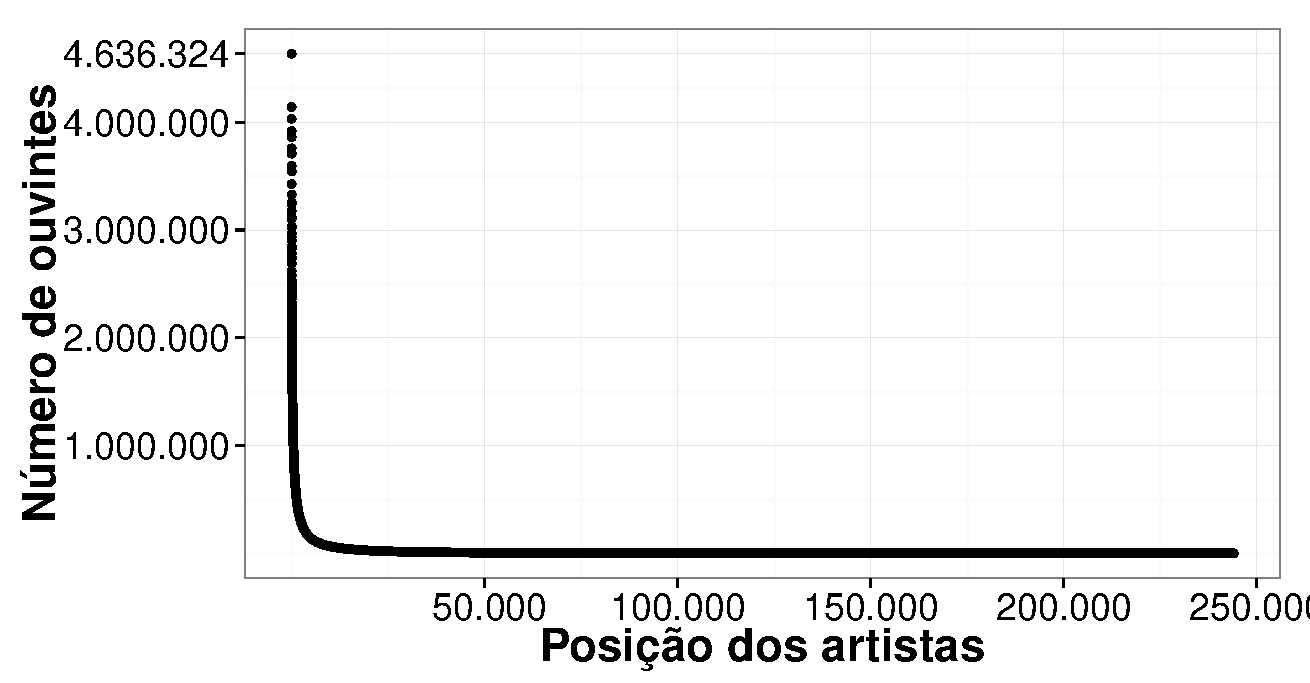
\includegraphics[scale=0.45]{figs/listeners.pdf}\label{fig:listeners}}\quad
  \subfigure[N�mero de ouvintes dos artistas (log linear)]{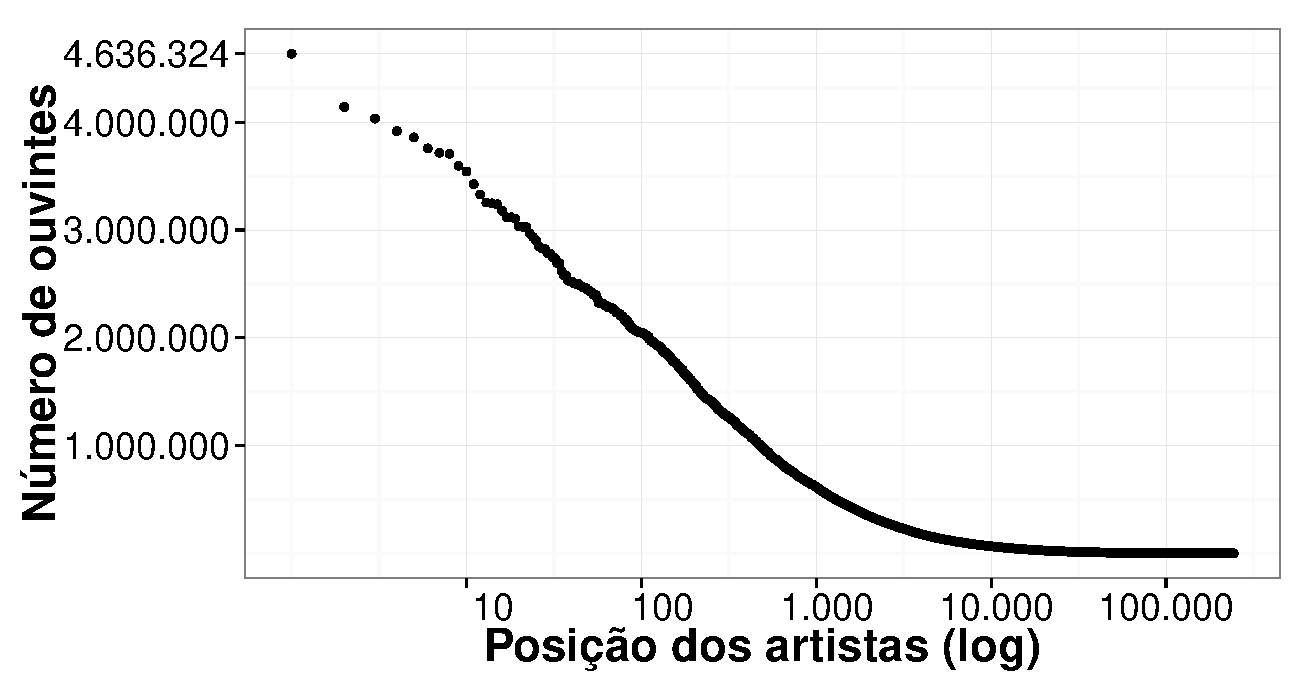
\includegraphics[scale=0.45]{figs/listeners_log.pdf} \label{fig:listeners_log} }
  \caption{N�mero de ouvintes dos artistas do Last.fm}
  \label{fig:listeners_lastfm}
\end{figure*}

A Figura \ref{fig:ecdf_pop} representa gr�ficos da distribui��o acumulada da popularidade dos artistas escutados pelos ouvintes. Podemos observar que os valores da popularidade dos artistas com novidade (Figura \ref{fig:ecdf_pop_new}) s�o em geral um pouco menores que os valores para os artistas conhecidos (Figura \ref{fig:ecdf_pop_old}).

\begin{figure}
\subfigure[Artistas com novidade]{
 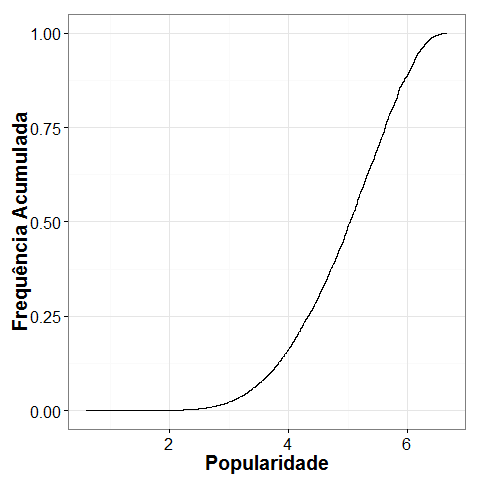
\includegraphics[width=.45\columnwidth]{figs/ecdf_n_pop.png} \label{fig:ecdf_pop_new}}
 \subfigure[Artistas conhecidos]{
 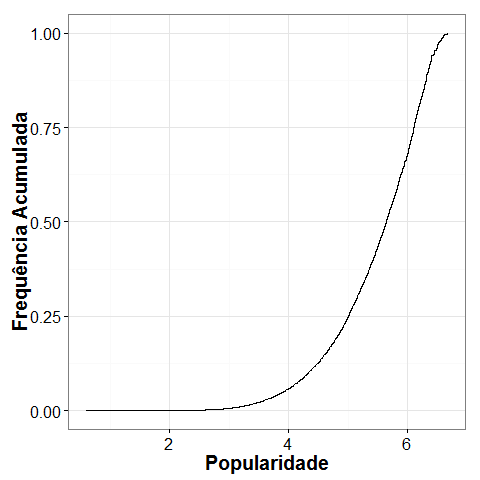
\includegraphics[width=.45\columnwidth]{figs/ecdf_old_pop.png}  \label{fig:ecdf_pop_old}}
  \caption{Frequ�ncia acumulada da popularidade dos artistas escutados pelos ouvintes (j� com valor transformado pelo log na base 10).}
  \label{fig:ecdf_pop}
\end{figure} 

	\section{Prefer�ncias}
	Para mensurar o quanto o ouvinte preferiu a novidade, foram utilizados duas m�tricas: a aten��o total e o per�odo de aten��o.  Como novidades podem ser descobertas em todo o Per�odo de Experimento, alguns destes artistas possuem uma janela de tempo no experimento menor (artistas escutadas no final do Per�odo de Experimento). Para contornar esse problema, utilizamos duas solu��es. Primeiro, utilizamos como denominador no c�lculo das m�tricas o n�mero de semanas da Janela de Tempo de exposi��o � novidade, que vai da primeira semana que foi escutada a novidade at� o fim do Per�odo de Experimento. Segundo, como mencionado na Se��o ~\ref{sec:timeline}, apenas as novidades descobertas no Per�odo de Observa��o foram consideradas na an�lise, mas todo o Per�odo de Experimento foi utilizado para c�lculo das m�tricas. Isso d� a cada novidade um m�nimo de 6 meses de coleta de dados, que limita um poss�vel vi�s para Janelas de Tempo pequenas.
	
		A aten��o total representa a aten��o que o ouvinte deu para o artista no Per�odo de Experimento. A aten��o total do ouvinte para o artista � representada pelo total de n�mero de execu��es de m�sicas do artista que ele escutou no Per�odo de Experimento, dividido pelo n�mero de semanas de sua Janela de Tempo. 
		
			J� o per�odo de aten��o o tempo que o ouvinte deu aten��o ao artista. Assim, � o n�mero de semanas que o ouvinte escutou o artista dividido pelo n�mero de semanas de sua Janela de Tempo.
	

\chapter{Prefer�ncias dos ouvintes para diferentes aspectos de novidades}\label{cap:pref}

Ap�s a coleta e filtragem dos dados, e da modelagem dos conceitos, partimos para responder as perguntas de pesquisa. Este cap�tulo abrange as duas primeiras perguntas, abordando as prefer�ncias dos ouvintes pelos aspectos - familiaridade e popularidade - da novidade, de forma geral e de forma individual.

\section{Prefer�ncias gerais}
Este trabalho visa entender como diferentes aspectos de novidades podem influenciar as prefer�ncias de ouvintes por elas. Para esta pesquisa, a primeira pergunta levantada foi: \textit{H� uma correla��o geral entre algum aspecto da novidade e as prefer�ncias dos ouvintes?} Para responder essa pergunta, calculamos a correla��o entre cada aspecto da novidade - familiaridade e popularidade - e cada m�trica de prefer�ncia - aten��o total e per�odo de aten��o, de todas as novidades de todos os ouvintes juntas. 

Com todas m�tricas das novidades em m�os, foi utilizado o m�todo de correla��o n�o-param�trico de Spearman. O resultado gerado por este m�todo pode variar de -1 a 1. Quanto mais pr�ximo de 1, mais as vari�veis est�o correlacionadas positivamente - se uma cresce/decresce a outra cresce/decresce. Quanto mais pr�ximo de -1, mais as vari�veis est�o correlacionadas negativamente - se uma cresce a outra decresce, e vice-versa. Se o valor estiver pr�ximo a 0 n�o h� correla��o. 

\begin{table} [htpb]
 \begin{center}
  
 \begin{tabular}{ |c|c|c|c| }
  \hline
  Dimens�es & F & P \\
  \hline
  Per�odo de aten��o (PdA)  & 0,08  & 0,07 \\
  Familiarity (F)   & -  & 0,08 \\
    \hline
      \end{tabular}
      \caption{Correla��o (Coeficiente de Spearman) entre aspectos da novidade e prefer�ncias, analisando todas as novidades juntas}\label{tab:correlations}
\end{center}
\end{table}
  
A tabela \ref{tab:correlations} mostra o coeficiente de Spearman para cada par de aspecto da novidade / prefer�ncia. Como pode-se ver, todos os valores encontrados da correla��o s�o pr�ximos de zero. \textbf{Podemos concluir que no geral n�o existe uma correla��o entre aspectos e prefer�ncias pela novidade, para todos os ouvintes juntos}. Por exemplo, os ouvintes em geral n�o preferem novidades familiares, ou no geral n�o preferem novidades n�o-familiares. N�s levantamos duas hip�teses para explicar esse resultado:

  

\begin{enumerate}
	\item Diferentes ouvintes possuem diferentes prefer�ncias para os aspectos das novidades.
	Nesta hip�tese, cogitamos que diferentes ouvintes possuem diferentes prefer�ncias musicais. Assim, existem ouvintes que preferem novidades populares, outros preferem novidades n�o populares, etc. Colocando todos estes ouvintes juntos, a correla��o geral vai ser pr�xima a zero.
	
	\item Individualmente, os ouvintes n�o preferem um aspecto a outro das novidades.
	Cada ouvinte pode preferir, por exemplo, tanto novidades familiares quanto n�o familiares, fazendo com que a correla��o entre a prefer�ncia e o aspecto das novidades seja pr�xima a zero.
\end{enumerate}

\section{Prefer�ncias individuais}

O resultado da primeira pergunta de pesquisa e estas hip�teses nos levam � segunda pergunta de pesquisa: individualmente, os ouvintes preferem algum aspecto de novidade? Para saber se os ouvintes possuem alguma correla��o entre os aspectos e as prefer�ncias das novidades, calculamos as correla��es para cada sujeito individualmente. Cerca de 74\% dos sujeitos possuem alguma correla��o com valor maior que 0,15 ou menor que -0,15, e cerca de 26\% possuem alguma correla��o maior que 0,3 ou menor que -0,3. Desta maneira, individualmente,  boa parte dos ouvintes possuem alguma correla��o entre algum aspecto e alguma prefer�ncia da novidade. A Figura \ref{fig:correlations_new} mostra a distribui��o acumulada dos valores das correla��es para cada par aspecto / prefer�ncia.

Analisando estes dois resultados juntos, pode-se concluir que, apesar de n�o existir uma tend�ncia geral quanto �s prefer�ncias dos sujeitos para os diferentes aspectos das novidades, \textbf{a maior parte dos sujeitos possuem alguma prefer�ncia para algum aspecto de novidade no seu comportamento}. Isso sugere a presen�a de diferentes tipos de ouvintes nos nossos dados. Para identificar estes tipos, foi utilizado um algoritmo de agrupamento nos sujeitos, que ser� discutido no pr�ximo cap�tulo. 

\begin{figure*}[htp]
  \centering
  \subfigure[Aten��o total e familiaridade]{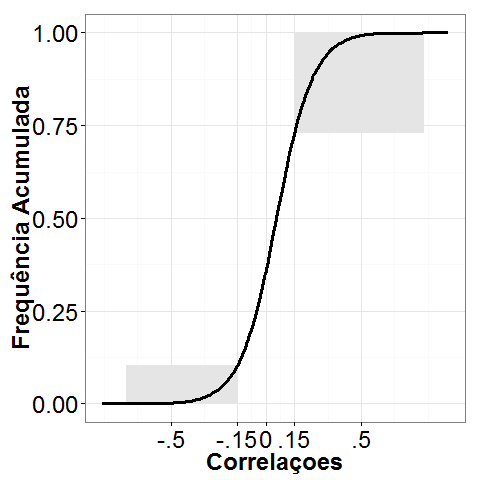
\includegraphics[scale=0.3]{figs/new_TA_F.png}}\quad
  \subfigure[Aten��o total e popularidade]{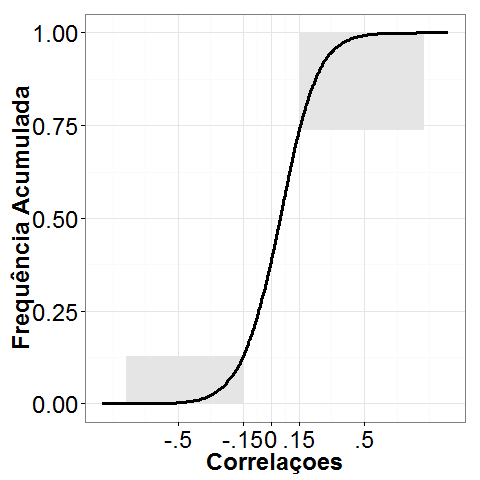
\includegraphics[scale=0.3]{figs/new_TA_P.png}}
  \subfigure[Per�odo de aten��o e familiaridade]{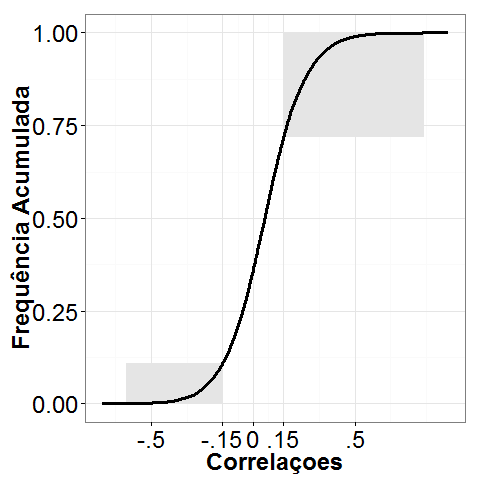
\includegraphics[scale=0.3]{figs/new_PA_F.png}}\quad
  \subfigure[Per�odo de aten��o e popularidade]{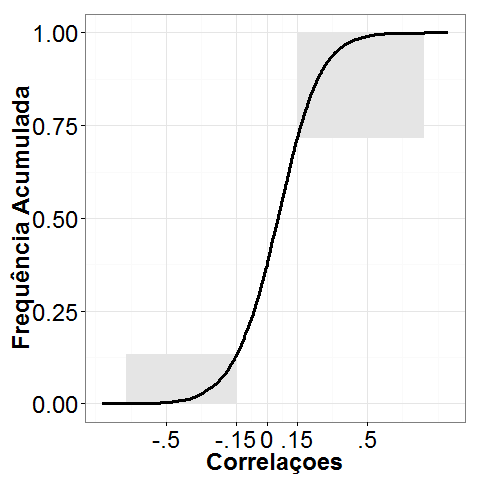
\includegraphics[scale=0.3]{figs/new_PA_P.png}}
  \caption{Distribui��o do coeficiente Spearman de correla��o entre os aspectos das novidades e as prefer�ncias de cada ouvinte dos dados. As �reas sombreadas representam a parte dos sujeitos com correla��o maior que 0.15 e menor que -0.15.}
  \label{fig:correlations_new}
\end{figure*}



\chapter{Grupos de usu�rios para diferentes aspectos de novidade} \label{sec:grupos}


De acordo com os resultados do Cap�tulo \ref{cap:pref}, h� a evid�ncia de diferentes tipos de sujeitos nos nossos dados, de acordo com as prefer�ncias pelos aspectos das novidades. Isto nos leva a terceira pergunta de pesquisa: Existem grupos de ouvintes relacionados com as prefer�ncias pelos aspectos das novidades baseadas no perfil? Para identificar estes grupos, foi realizado um agrupamento nos dados que caracterizam os sujeitos. Esta an�lise ser� descrita neste cap�tulo.

%%%%%%%%%%%%%%%%%%%%%%%%%%%%%%%%%%%%%%%%%%%%%%%%%%%%%%%%%%%%%%%%%%%%%%%%%%%%%%
%%%%%%%%
%%%%%%%%%%%%%%%%%%%%%%%%%%%%%%%%%%%%%%%%%%%%%%%%%%%%%%%%%%%%%%%%%%%%%%%%%%%%%%
\section{Conjunto de sujeitos}
Primeiramente, a an�lise foi realizada com os dados dos mesmos sujeitos utilizados na an�lise das prefer�ncias dos ouvintes para os aspectos das novidades (Cap�tulo ~\ref{cap:pref}). Depois, para estudar especificamente os sujeitos com alguma correla��o entre prefer�ncia e aspectos da novidade, foi feita a an�lise com dois subconjuntos: o primeiro subconjunto consiste em sujeitos com valor de correla��o entre algum aspecto e prefer�ncia da novidade maior que 0,15 ou menor que -0,15; o segundo consiste em sujeitos com valor de correla��o maior que 0,3 ou menor que -0,3. Os resultados encontrados nas tr�s an�lises foram similares. Portanto, mostraremos apenas os resultados da primeira an�lise.%, enquanto os outros resultados est�o no ap�ndice \lma{X}.%


%%%%%%%%%%%%%%%%%%%%%%%%%%%%%%%%%%%%%%%%%%%%%%%%%%%%%%%%%%%%%%%%%%%%%%%%%%%%%%
%%%%%%%%
%%%%%%%%%%%%%%%%%%%%%%%%%%%%%%%%%%%%%%%%%%%%%%%%%%%%%%%%%%%%%%%%%%%%%%%%%%%%%%
\section{Dados que caracterizam sujeitos} \label{sec:dadosCaracterizam}
O objetivo da an�lise atual � identificar os grupos de ouvintes baseados nas prefer�ncias pelos aspectos das novidades comparadas com seus h�bitos musicais. A ideia de investigar as m�tricas relacionadas �s novidades e aos h�bitos musicais � para saber se o comportamento do ouvinte por novidade � semelhante ao seu comportamento no geral. Foram escolhidas 5 m�tricas de caracteriza��o dos sujeitos, que podem ser divididas em dois grupos: m�tricas relacionadas com novidades e m�tricas relacionadas com os h�bitos musicais.

\begin{enumerate}
	\item \textbf{Relacionadas com novidades}: 	M�tricas que caracterizam os sujeitos a partir de suas prefer�ncias pelos aspectos das novidades.
	
\begin{itemize}
	\item \textit{Correla��o entre a familiaridade das novidades e a aten��o total dedicada a elas durante o experimento.}
		\item \textit{Correla��o entre popularidade das novidades e a aten��o total dedicada a elas durante o experimento.}
\end{itemize}

\textit{*Calculamos a correla��o (coeficiente de Spearman) entre a aten��o total e o per�odo de aten��o, e o valor encontrado foi de 0,71. Como ambas as vari�veis est�o correlacionadas, decidimos utilizar no algoritmo de agrupamento apenas as correla��es que envolvem a aten��o total.}

	\item  \textbf{Relacionadas com os h�bitos musicais}: M�tricas que caracterizam os h�bitos musicais do sujeito e que podem ser contrastadas com as m�tricas das novidades.
	
	\begin{itemize}
	\item \textit{Ecleticidade} A ecleticidade representa o qu�o diferente os artistas do perfil do ouvinte s�o, de acordo com seus descritores. Sua defini��o e c�lculo foi feito na Subse��o ~\ref{subsec:eclet}. A ecleticidade est� relacionada com a familiaridade da novidade, pois quanto mais ecl�tico um sujeito for, maior a probabilidade dele ser familiar a v�rios tipos de novidades.
	
		\item \textit{Popularidade m�dia dos artistas do perfil do ouvinte} Esta m�trica � �til para comparar com a popularidade das novidades escutadas pelo ouvinte.
		
			\item \textit{Propor��o de novidades escutadas pelo ouvinte no Per�odo de Observa��o} Com esta m�trica pode-se identificar se o ouvinte possuiu o h�bito de escutar muitas ou poucas novidades, no Per�odo de Observa��o.
\end{itemize}

\end{enumerate}


\section{Algoritmo de agrupamento}
Para fazer o agrupamento dos sujeitos foi utilizado o algoritmo de agrupamento aglomerativo hier�rquico. Como descrito na Se��o ~\ref{sec:perfil}, este tipo de algoritmo necessita de uma m�trica de dissimilaridade entre os pares de sujeitos e um crit�rio de uni�o que especifica quais grupos unir em cada passo. 

Para calcular a dissimilaridade entre os sujeitos, primeiro foram calculadas as m�tricas descritas na Se��o ~\ref{sec:dadosCaracterizam}. Ap�s o c�lculo, estes dados foram normalizados, baseados no Z-Score. Ent�o, a  dissimilaridade entre dois sujeitos foi calculada a partir da dist�ncia euclidiana, onde cada sujeito � representado por um vetor contendo as 5 m�tricas normalizadas. Formalmente, sejam $S$ o conjunto de vetores com dados normalizados que representam cada sujeito; e $x\in S$ e $y\in S$ vetores de dois sujeitos de $S$. $x_i$ representa a posi��o $i$ do vetor $x$, no caso uma das 5 m�tricas que caracterizam os sujeitos. A dissimilaridade entre os sujeitos, representada pela dissimilaridade $	\text{disSuj}(x,y) $ dos vetores que os representam � dado pela Equa��o \ref{eq:a}. Como crit�rio de uni�o, foi utilizado o m�todo Ward \cite{Ward63}. 

\begin{equation}
	\text{disSuj}(x,y) =  \sqrt{ \sum_{i=1}^5 (x_{i} - y_{i})^2} \label{eq:a}
\end{equation}



\section{Escolha do n�mero de grupos}

O m�todo de agrupamento hier�rquico n�o exp�e explicitamente o n�mero de grupos resultantes. A cada passo, o algoritmo une dois grupos, at� que todos os sujeitos estejam em um s� grupo.	Uma abordagem para definir a melhor configura��o de n�mero de grupos � o m�todo do joelho \cite{Thorndike}, ao plotar um gr�fico onde o eixo X � o n�mero de grupos e o Y um crit�rio de avalia��o. A Figura \ref{fig:hetero} mostra a dist�ncia m�dia dentro dos grupos para cada configura��o de n�mero de grupos. O m�todo de joelho determina escolher uma configura��o de grupos que n�o adicionem muita heterogeneidade, evidenciado a partir da curvatura m�xima do gr�fico (joelho). Pela figura, a dist�ncia m�dia dentro dos grupos come�a a aumentar vertiginosamente nas configura��es com menos de 7 grupos. Assim, analisamos as configura��o com 7 e 8 grupos.

\begin{figure}[htbp]
\center
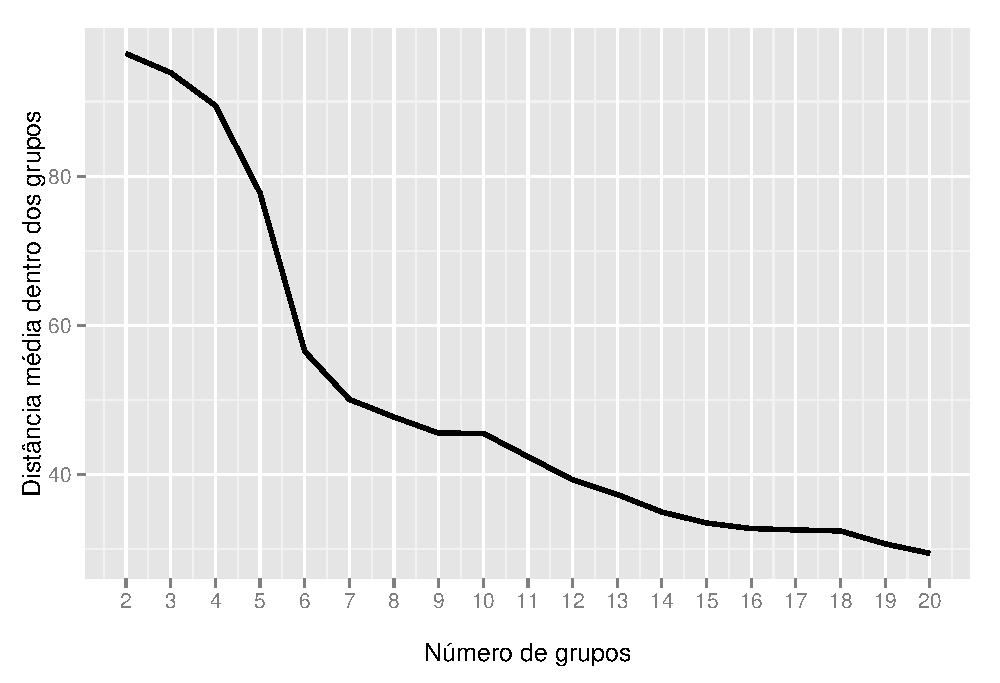
\includegraphics[width=0.7\columnwidth]{media.pdf}
\caption{N�mero de grupo X Dist�ncia m�dia dentro dos grupos. O joelho do gr�fico est� em torno da configura��o com 7 grupos.}
  \label{fig:hetero}
\end{figure} 

A Tabela \ref{tab:tab} mostra os valores dos centr�ides para a solu��o de 7 grupos e o centr�ide criado na solu��o de 8 grupos (Centr�ide 8). Como podemos ver, o Centr�ide 2 � similar ao Centr�ide 8. Desta maneira, escolhemos a configura��o com 7 grupos.

\begin{table} 
 \begin{center}
  
\pgfplotstabletypeset[
    col sep=semicolon,
    string type,
    every head row/.style={before row=\hline,after row=\hline},
    every last row/.style={after row=\hline},
    every first column/.style={
		column type/.add={|}{}
		},
		every last column/.style={
		column type/.add={}{|}
		}]
     {centroides_latex.csv}     
      \caption{Centr�ides para as configura��es com 7 grupos e com 8 grupos}
      \label{tab:tab}
    \end{center}
\end{table}

%","","","media pop","prop novid

\section{Grupos}
Ap�s a escolha de 7 grupos de ouvintes, utilizamos o centr�ide de cada grupo para analisar as suas principais caracter�sticas.  A Figura \ref{fig:clusters} representa os valores dos centr�ides normalizados. 
Podemos dividir os grupos em dois tipos: o primeiro, onde as caracter�sticas que se destacam s�o as relacionadas com as prefer�ncias pelos aspectos das novidades e o segundo, onde as caracter�sticas que se destacam s�o as relacionadas com os h�bitos musicais dos ouvintes. De acordo com cada centr�ide, rotulamos os grupos da seguinte forma:

\begin{figure}[htbp]
\centering
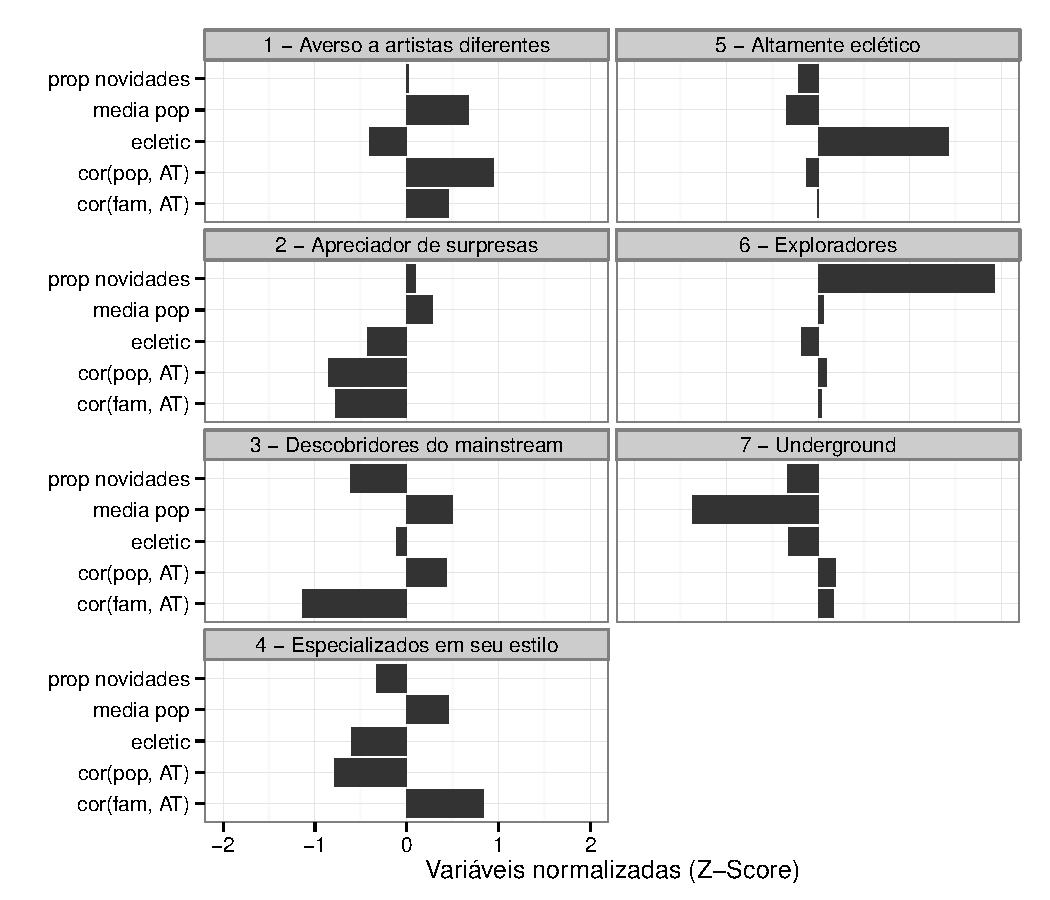
\includegraphics[scale=1]{clusterstodos1.pdf}
\caption{Centr�ides dos 7 grupos encontrados na an�lise. As m�tricas est�o normalizadas pelo z-score, onde zero representa a m�dia de todos os ouvintes, e a unidade de varia��o � um desvio padr�o, para cada m�trica. No eixo vertical, \textit{fam} significa a familiaridade, \textit{pop} significa popularidade, \textit{AT} significa aten��o total.}
  \label{fig:clusters}
\end{figure} 

%total: 11.449
\begin{enumerate}
	\item Grupos marcados pelas prefer�ncias pelos aspectos das novidades
	\begin{enumerate} 
		\item Averso a artistas diferentes (ou acomodado) [total de ouvintes: 2317 (20\%)]: Maior grupo com caracter�stica marcante pelas prefer�ncias pelos aspectos das novidades, formado por ouvintes que preferem novidades familiares e populares, al�m de possu�rem h�bitos musicais marcados por artistas populares.
		\item Apreciador de surpresas [total de ouvintes: 1859 (17\%)]: Ouvintes preferem novidades n�o-familiares e pouco populares. 
		\item Descobridores do mainstream [total de ouvintes: 1022 (8\%)]: Ouvintes que preferem novidades n�o-familiares e populares.
		\item Especializados em seu estilo [total de ouvintes: 1467 (14\%)]: Ouvintes que preferem novidades pouco populares e familiares, al�m de possuirem pouca ecleticidade.
	
	\end{enumerate}
	\item Grupos marcados pelas caracter�sticas dos h�bitos musicais
	\begin{enumerate}
		\item Altamente ecl�tico [total de ouvintes: 2456 (21\%)]: Maior grupo de todos, formado por ouvintes que possuem alta ecleticidade
		\item Exploradores [total de ouvintes: 1047 (9\%)]: Ouvintes que possuem alta propor��o de novidades escutadas durante o Per�odo de Observa��o
		\item Underground [total de ouvintes: 1281 (11\%)]: Ouvintes com h�bito musical marcado por artistas pouco populares.
	\end{enumerate}
\end{enumerate}

\section{Discuss�o dos grupos encontrados}

Encontramos 4 grupos que possuem como caracter�sticas marcantes as prefer�ncias pelos aspectos das novidades. Coincidentemente, foram encontrados grupos com todas as combina��es poss�veis de prefer�ncias pelos aspectos. 

O maior destes 4 grupos � o que chamamos \textit{Averso a artistas diferentes}. � um grupo de ouvintes que preferem novidades familiares e populares, al�m de possu�rem h�bitos musicais marcados por artistas populares, pouca ecleticidade e propor��o mediana de novidades escutadas. � um tipo de ouvinte que n�o procura expandir seu perfil musical, preferindo escutar o que est� na m�dia do que ele habitualmente j� escuta. A Figura \ref{fig:tudo_alto} representa o perfil de um ouvinte \textit{Averso a artistas diferentes}. Nota-se que as novidades mais preferidas s�o as mais familiares e mais populares.

\begin{figure}[htbp]
\center
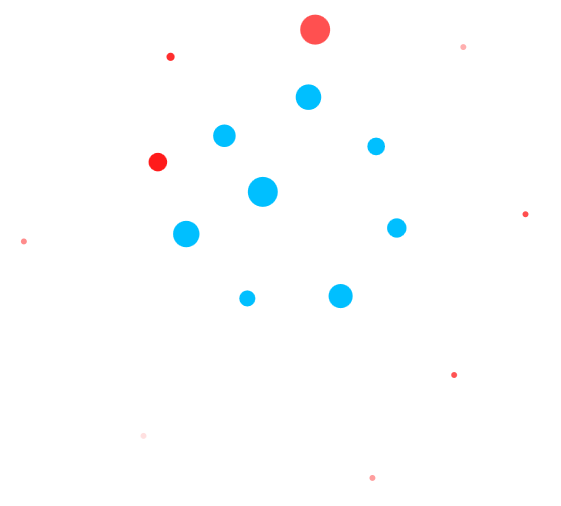
\includegraphics[width=0.5\columnwidth]{figs/alto_tudo.png}
\caption{Perfil de um ouvinte \textit{Averso a artistas diferentes}. Os c�rculos azuis s�o os clusters e os vermelhos as novidades. A opacidade dos c�rculos vermelhos est� relacionada com a prefer�ncia do ouvinte pela novidade em quest�o. As novidades mais preferidas s�o as mais familiares e populares.}
  \label{fig:tudo_alto}
\end{figure} 

\begin{figure}[htbp]
\center
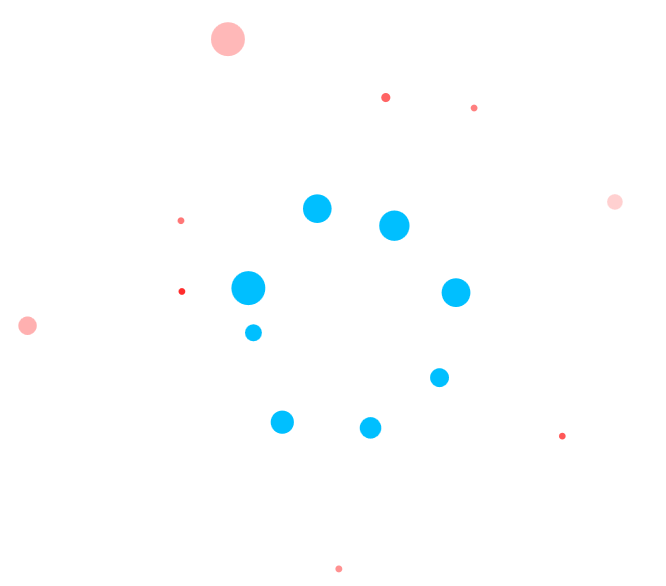
\includegraphics[scale=0.9]{figs/baixo_tudo.png}
\caption{Perfil de um ouvinte \textit{Apreciador de surpresas}. As novidades mais preferidas s�o as menos familiares e menos populares.}
  \label{fig:baixo_tudo}
\end{figure} 

Os outros 3 grupos dos marcados pelas prefer�ncias pelos aspectos das novidades possuem uma distribui��o mais homog�nea do n�mero de ouvintes. Opostos aos \textit{Aversos a artistas diferentes}, os \textit{Apreciadores de surpresas} preferem novidades n�o familiares e n�o populares, al�m de possuir pouca ecleticidade. Desta maneira, estes ouvintes normalmente escutam artistas bem parecidos, mas tentam aumentar esse leque de artistas do perfil preferindo novidades n�o familiares e n�o populares. Eles preferem surpresas, artistas diferentes do que j� escutaram. A Figura \ref{fig:baixo_tudo} representa o perfil de um ouvinte \textit{Apreciador de surpresas}. Nota-se que as novidades mais preferidas s�o  as menos familiares e menos populares.


Os \textit{Descobridores do mainstream} preferem novidades populares, que est�o na m�dia, mesmo n�o sendo familiares. Uma poss�vel explica��o seria ouvintes que escutam o que est� nas paradas das r�dios, sem se importar se s�o parecidos com o que ele escutava antes ou n�o. J� os \textit{Especializados em seu estilo} preferem novidades familiares e pouco populares, al�m de possu�rem pouca ecleticidade. Esse tipo de ouvinte s�o fechados no seu nicho de estilos musicais, e ou n�o preferem o que est� na m�dia destes estilos, ou j� escutaram tudo que est� na m�dia e agora querem expandir para artistas n�o populares destes estilos.

Analisando os 3 grupos restantes, o \textit{Altamente ecl�tico} � o grupo de ouvintes com maior ecleticidade, comparando com os demais. Nota-se que neste grupo existem diferentes sujeitos, por que as outras m�tricas s�o pr�ximas a zero. O grupo de \textit{Exploradores}, formado por ouvintes com alta propor��o de novidades escutadas no per�odo de observa��o, tamb�m possui essa caracter�stica do \textit{Altamente ecl�tico}. Por fim, o grupo \textit{Underground} � formado por ouvintes que t�m h�bito de escutar artistas pouco populares no geral.

\chapter{Compara��o das novidades com os artistas conhecidos}\label{cap:comparacao}

At� este momento trabalhamos apenas com novidades. Por�m, ser� que as prefer�ncias dos ouvintes pelas novidades s�o as mesmas que pelos artistas conhecidos? Caso esta hip�tese seja verdade, o comportamento dos ouvintes para estes dois �mbitos, novidades e n�o-novidades, seriam similares, podendo estender os resultados das novidades para os itens conhecidos e vice-versa. Para responder esta pergunta expandimos nossos experimentos para englobar tamb�m os artistas conhecidos, tentando responder a seguinte pergunta de pesquisa: \textit{As rela��es entre as prefer�ncias dos ouvintes e os aspectos das novidades s�o as mesmas que as rela��es entre as prefer�ncias dos ouvintes e os aspectos dos artistas j� conhecidos?}

\section{Sele��o de sujeitos}
Para esta an�lise, utilizamos os mesmos 11.989 sujeitos das an�lises anteriores e aplicamos um filtro, para selecionar os sujeitos que foram expostos a um n�mero m�nimo de artistas conhecidos que permitisse a investiga��o de rela��es entre as caracter�sticas destes artistas e as prefer�ncias. Filtro similar foi descrito na Se��o \ref{sec:Filtros} para a sele��o de sujeitos que foram expostos a um n�mero m�nimo de novidades.

Desta maneira, foram exclu�dos os usu�rios que escutaram menos de 10 artistas conhecidos no Per�odo de Observa��o. Ap�s esta exclus�o ficamos com uma amostra de 10.207 sujeitos para os experimentos.

\section{Caracter�sticas dos artistas conhecidos}\label{sec:comp_carac}
		
Como dito na Se��o \ref{sec:timeline}, os artistas conhecidos s�o os artistas escutados no Per�odo de Observa��o que j� foram escutados previamente no Hist�rico Inicial do ouvinte. Para eles foram calculadas 3 das 4 m�tricas que foram calculadas para os artistas com novidade (Cap�tulo \ref{cap:modelos}): familiaridade e popularidade (aspectos) e total de aten��o (prefer�ncia).

Para calcular as rela��es entre os aspectos dos artistas conhecidos e as prefer�ncias pelos ouvintes, utilizamos a mesma metodologia descrita no Cap�tulo \ref{cap:pref}. Utilizamos o m�todo de correla��o n�o-param�trico de Spearman entre cada par de aspecto / prefer�ncia.

\section{Compara��o entre rela��es das prefer�ncias e aspectos das novidades e dos artistas conhecidos}\label{sec:comp_pref}
Para guiar nossos experimentos, decidimos especificar a quarta pergunta de pesquisa, que � mais gen�rica. Assim, tentamos responder duas perguntas de pesquisa. 

	A primeira \textit{As rela��es entre as prefer�ncias dos ouvintes e os aspectos das novidades s�o significantemente diferentes das rela��es entre as prefer�ncias dos ouvintes e os aspectos dos artistas j� conhecidas?}	Se as rela��es comparadas forem significantemente iguais, poder�amos estender os resultados das novidades para o comportamento geral do ouvinte. Se forem diferentes, corroboraremos a import�ncia da an�lise separada de itens com novidades e itens conhecidos.

Para cada um dos 10.207 sujeitos foram calculados os valores das correla��es entre a familiariade e o total de aten��o e entre a popularidade e o total de aten��o, tanto para os artistas com novidade quanto para os artistas conhecidos. Os detalhes destes c�lculos foram apresentados no Cap�tulo \ref{cap:pref} e na Se��o \ref{sec:comp_carac}. Desta maneira cada ouvinte possui pares de correla��es (Tabela \ref{tab:correlacoes_nov_con}), onde um valor do par � referente aos artistas com novidade e o outro os artistas conhecidos. Por exemplo, cada ouvinte possui um valor de correla��o entre a familiaridade e o total de aten��o para as novidades e um valor de correla��o entre a familiaridade e o total de aten��o para os artistas conhecidos. 

Desta maneira, para responder a pergunta exposta no par�grafo anterior, utilizamos um teste-T pareado, para cada par de correla��o novidade / artista conhecido correspondente de todos os ouvintes. O intuito desta an�lise � descobrir se, por exemplo, o valor da correla��o entre a familiaridade e o total de aten��o para as novidades e para os artistas conhecidos s�o significantemente diferentes. 

\begin{table} [htpb]
 \begin{center}
  
 \begin{tabular}{ |c|c| }
  \hline
  Artistas com novidade & Artistas conhecidos \\
  \hline
 cor( familiaridade, aten��o total ) &   cor( familiaridade, aten��o total ) \\    \hline
 cor( popularidade, aten��o total ) &  cor( popularidade, aten��o total ) \\    \hline
      \end{tabular}
      \caption{Correla��es calculadas para artistas com novidade e artistas conhecidos.}\label{tab:correlacoes_nov_con}
\end{center}
\end{table}

A Tabela \ref{tab:testeT} mostra o p-valor e o intervalo de confian�a da m�dia das diferen�as para cada par de aspecto / prefer�ncia. Em ambas m�tricas comparadas, a probabilidade da m�dia das diferen�as entre os valores para os artistas com novidade e os artistas conhecidos ser igual a zero � baix�ssima (p-valor <  0.0001). Desta maneira, podemos afirmar que as correla��es no geral s�o diferentes. Ou seja, as rela��es dos ouvintes entre as prefer�ncias e os aspectos, para artistas com novidade e artistas conhecidos, s�o diferentes.


\begin{table} [htpb]
 \begin{center}
  
 \begin{tabular}{ |c|c|c|c| }
  \hline
  M�tricas & P-Valor & Intervalo de Confian�a ($\alpha$ = 0.05) \\
  \hline
  Familiaridade / Per�odo de aten��o  & < 0.0001  & [-0,14 -0,13] \\
  Popularidade / Per�odo de aten��o   & < 0.0001  & [-0,04 -0,03]\\
    \hline
      \end{tabular}
      \caption{Teste-T pareado entre as correla��es dos aspectos e prefer�ncias dos ouvintes para artistas com novidade e artistas conhecidos.}\label{tab:testeT}
\end{center}
\end{table}

Outro fato que podemos observar da tabela � que o intervalo de confian�a, com 95\% de confian�a, para as diferen�as das correla��es entre familiaridade e aten��o total para artistas com novidade e artistas conhecidos � [-0,14 -0,13], sugerindo que as prefer�ncias pelos artistas conhecidos familiares s�o maiores que as prefer�ncias pelos artistas com novidade familiares. Uma poss�vel explica��o seria que os artistas conhecidos mais familiares s�o os artistas que o ouvinte mais escutou no seu hist�rico. Assim, naturalmente a prefer�ncia por eles � bem maior.

J� o intervalo de confian�a, com 95\% de confian�a, para as diferen�as das correla��es entre popularidade e aten��o total para artistas com novidade e artistas conhecidos � [-0,04 -0,03]. Tamb�m sugere que as prefer�ncias pelos artistas mais populares conhecidos s�o maiores que pelos artistas mais populares com novidade, apesar de que este intervalo de confian�a est� mais pr�ximo de zero que o intervalo de confian�a anterior.

No geral, podemos concluir que as prefer�ncias dos ouvintes por artistas mais familiares e mais populares � menor se os artistas forem novidades do que se eles forem artistas conhecidos. � como se a prefer�ncia por artistas conhecidos j� esteja consolidada e que ao escutar novidades os ouvintes tendem a explorar mais, escutando no mesmo per�odo de tempo mais artistas menos familiares e menos populares que os artistas conhecidos.


J� a segunda pergunta de pesquisa, \textit{Existe correla��o entre as rela��es das prefer�ncias pelos aspectos dos artistas com novidade e as rela��es das prefer�ncias pelos aspectos dos artistas conhecidos?}
Pr�ximo passo foi verificar se existiam correla��es entre as rela��es calculadas para os artistas com novidade e para os artistas conhecidos. Ser� que quanto maior a correla��o de um ouvinte entre familiaridade e aten��o total para artistas com novidade, por exemplo, maior a correla��o entre a familiaridade e aten��o total para artistas conhecidos? Para responder a pergunta de pesquisa, utilizamos o m�todo de correla��o n�o-param�trico de Spearman.


\begin{table} [htpb]
 \begin{center}
  
 \begin{tabular}{ |c|c|c|c| }
  \hline
  Novidades X Artistas conhecidos & cor(fam., aten. tot.) & cor(pop. , aten. tot.) \\
  \hline
  cor(familiaridade , aten��o total)  & 0,05  & -0.02 \\
  cor(popularidade , aten��o total)   &  -0.04 & 0,09 \\
    \hline
      \end{tabular}
      \caption{Correla��o (Coeficiente de Spearman) entre correla��es calculadas para novidades (linhas) e artistas conhecidos (colunas)}\label{tab:comp_cor}
\end{center}
\end{table}
  
 Como podemos observar na Tabela \ref{tab:comp_cor}, a correla��o � baixa em todos os casos. N�o podemos afirmar, por exemplo, que dado dois ouvintes, se um possuir maior correla��o entre familiaridade e per�odo de aten��o para novidades que o outro ouvinte ele ter� maior chance de ter maior correla��o entre familiaridade e per�odo de aten��o para artistas conhecidos, e vice-versa. 
 
 Esta falta de correla��o geral pode ser ocasionada pela diversidade de comportamentos para novidades e artistas conhecidos dos ouvintes. Levantamos a hip�tese de que, por exemplo, existem ouvintes que possuem uma prefer�ncia mais forte por novidades familiares que por artistas conhecidos familiares, enquanto outros n�o. Hip�tese semelhante a esta foi exposta no Cap�tulo \ref{cap:pref}, que nos levou a criar perfis de ouvintes baseados nas rela��es entre prefer�ncias e os aspectos das novidades (Capitulo \ref{sec:grupos}). Desta maneira, fizemos uma investiga��o parecida para testar a hip�tese. 
 


\section{Grupos de ouvintes baseados na diferen�a das rela��es entre prefer�ncias e aspectos das novidades e dos artistas conhecidos}

Como as correla��es encontradas na segunda pergunta de pesquisa da se��o anterior foram baixas, seguindo a metodologia dos Cap�tulos \ref{cap:pref} / \ref{sec:grupos} tentamos encontrar perfis de ouvintes, com o intuito de responder a seguinte pergunta: \textit{Quais os diferentes perfis de ouvintes baseados nas diferen�as das rela��es prefer�ncias / aspectos das novidades e dos itens conhecidos?}

Primeiro passo foi calcular duas diferen�as, para cada ouvinte: primeiro, a diferen�a entre as correla��es da familiaridade e aten��o total das novidades e dos artistas conhecidos (linha 1 da Tabela \ref{tab:correlacoes_nov_con}) e segundo, a diferen�a entre as correla��es da popularidade e aten��o total das novidades e dos artistas conhecidos (linha 2 da Tabela \ref{tab:correlacoes_nov_con}) .	

Com estas diferen�as em m�os utilizamos o algoritmo de agrupamento aglomerativo hier�rquico. A escolha do n�mero de grupos foi baseada no m�todo do joelho. Na imagem \ref{fig:height_diferenca} podemos observar um in�cio de joelho entre as configura��es com 4 e 6 grupos. Comparando os centr�ides das configura��es de 6 e 7 grupos (Tabela \ref{tab:centroides_grupos_old}), podemos notar que o centr�ide adicionado na configura��o de 7 grupos (Centr�ide 7) � similar ao Centr�ide 5. Assim, como adicionar um
grupo na configura��o 6 n�o muda muito, escolhemos a configura��o de 6 grupos.

\begin{figure}[htbp]
\center
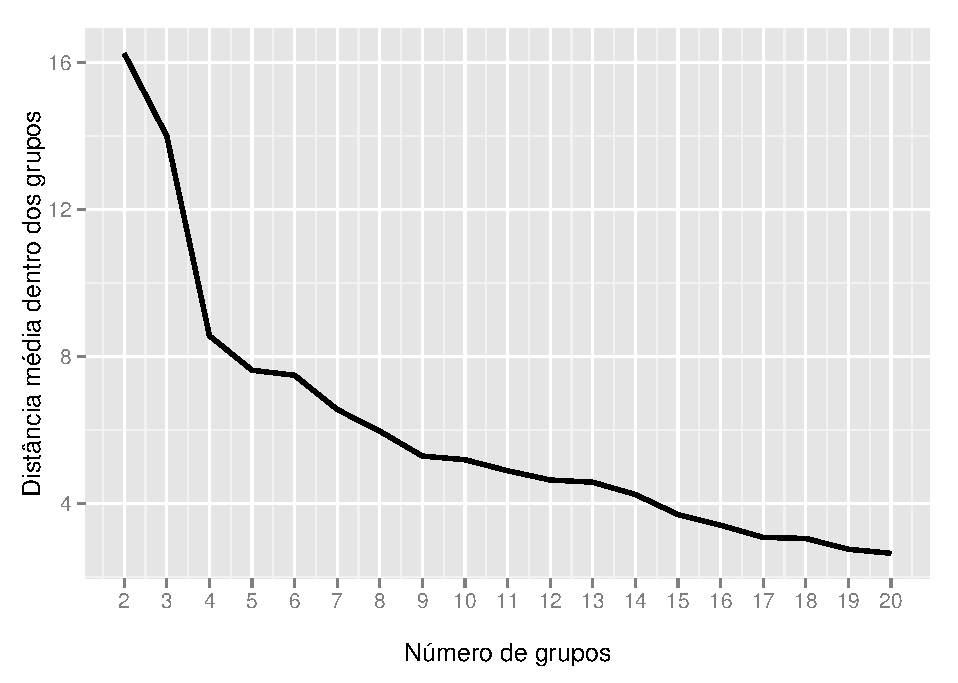
\includegraphics[width=0.7\columnwidth]{height_diferenca.pdf}
\caption{N�mero de grupo X Dist�ncia m�dia dentro dos grupos.}
  \label{fig:height_diferenca}
\end{figure} 

\begin{table} 
 \begin{center}
  
\pgfplotstabletypeset[
    col sep=semicolon,
    string type,
    every head row/.style={before row=\hline,after row=\hline},
    every last row/.style={after row=\hline},
    every first column/.style={
		column type/.add={|}{}
		},
		every last column/.style={
		column type/.add={}{|}
		}]
     {centroides_old.csv}     
      \caption{Centr�ides para a configura��o com 6 grupos e com 7 grupos}
      \label{tab:centroides_grupos_old}
    \end{center}
\end{table}

Ap�s a escolha dos 6 grupos de ouvintes, utilizamos o centr�ide de cada grupo para analisar as suas principais caracter�sticas.  A Figura \ref{fig:clusters_diferenca} representa os valores dos centr�ides. 

\begin{figure}[htbp]
\center
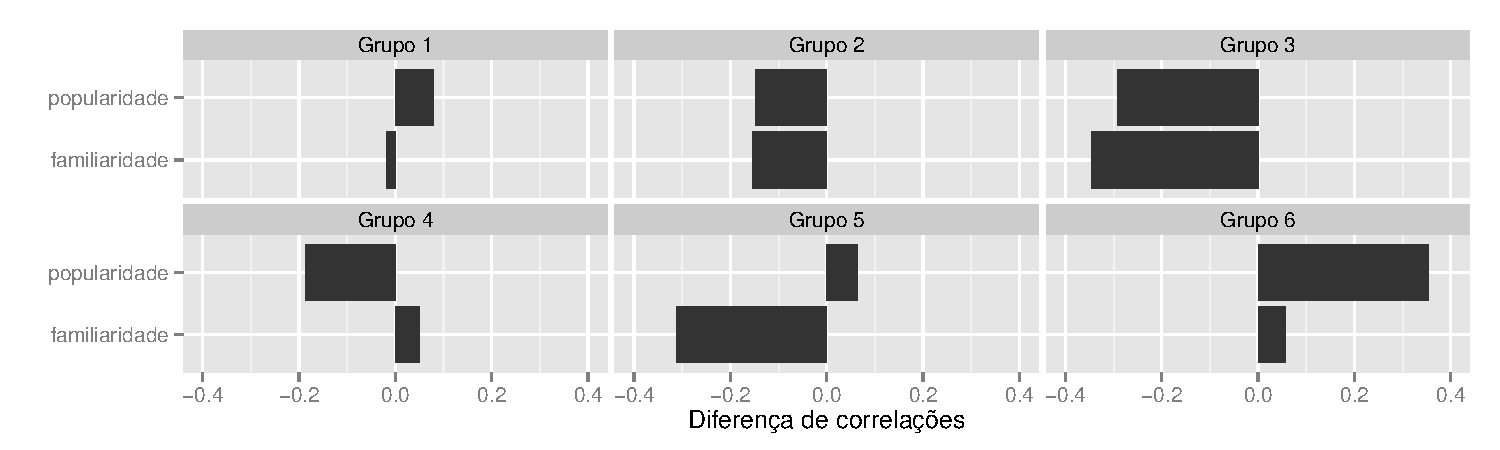
\includegraphics[width=1.0\columnwidth]{clusters_diferenca.pdf}
\caption{Centr�ides dos 6 grupos encontrados na an�lise da diferen�a das correla��es}
  \label{fig:clusters_diferenca}
\end{figure} 


Podemos dividir os grupos em quatro tipos: 
\begin{enumerate}
	\item Tipo I - Prefer�ncias similares para novidades e itens conhecidos [total de ouvintes: 2.427 (23\%)]: Composto pelo grupo 1, o centroide deste evidencia que as diferen�as entre as correla��es, dos dois pares de prefer�ncia / aspecto, calculadas para novidades e itens conhecidos, s�o pr�ximas a zero.  %\lma{colocar exemplo de ouvinte?}%
	\item Tipo II - Correla��es para itens conhecidos maiores que para novidades [total de ouvintes: 2.833 (27.7 \%)]: O segundo tipo � composto pelos grupos 2 e 3, onde as correla��es, dos dois pares de prefer�ncia / aspecto, s�o maiores para os itens conhecidos que para as novidades, seja em maior (grupo 2) ou menor (grupo 3) grau.% \lma{exemplo}%
	\item Tipo III - Correla��o para itens conhecidos maior que para novidades em apenas um aspecto [total de ouvintes: 4.529 (44.3 \%)]: composto pelos grupos 4 e 5, apenas um par prefer�ncia / aspecto possui correla��o para itens conhecidos maior que para novidades, enquanto que o outro par � pr�ximo a zero. O grupo 4 � formado no geral por ouvintes que possuem correla��es entre prefer�ncia e familiaridade para itens conhecidos maiores que para novidades. J� o grupo 5 � formado no geral por ouvintes que possuem correla��es entre prefer�ncia e popularidade para itens conhecidos maiores que para novidades.% \lma{exemplo}%
	\item Tipo IV - Correla��o das prefer�ncias e popularidade para novidades maior que para itens conhecidos [total de ouvintes: 418 (5\%)]: por �ltimo, este tipo de ouvinte possui correla��o entre prefer�ncia e popularidade maior para novidades que para artistas conhecidos. Composto pelo grupo 6.
	
	Boa parte dos grupos (4 dos 6) s�o formados no geral por ouvintes que possuem pelo menos correla��o de algum par prefer�ncia / aspecto maior para itens conhecidos que para novidades. Isso corrobora os resultados encontrados na Se��o \ref{sec:comp_pref}, que mostra que no geral os ouvintes possuem correla��es maiores para itens conhecidos que para novidades. Cerca de 23\% dos ouvintes est�o no grupo de comportamento parecido para novidades e itens conhecidos. Assim, poder�amos tentar prever comportamento para novidades baseados no comportamento de itens conhecidos para apenas 1/4 dos ouvintes, enquanto os demais precisariam de um tratamento diferenciado para estes dois tipos de comportamentos.
	
	% 2427 + 418 + 1256 + 1855 + 2674+ 1577 = 10207
\end{enumerate}
\chapter{Conclus�o}
Neste cap�tulo apresentamos um resumo geral da nossa pesquisa sobre os aspectos e prefer�ncias das novidades musicais. A partir deste resumo, discutimos os resultados obtidos e as implica��es. %Por fim expomos as limita��es do trabalho.

\section{Resumo}
O principal objetivo da pesquisa foi analisar as novidades de forma multidimensional, de acordo com dois aspectos - a popularidade e a familiaridade. A an�lise foi feita relacionando estes aspectos com as prefer�ncias dos ouvintes pelas novidades.

Na primeira parte da pesquisa analisamos as correla��es entre as prefer�ncias dos ouvintes e os aspectos das novidades, para as novidades de todos os sujeitos juntos. Foi descoberto que n�o h� uma correla��o entre as prefer�ncias e os aspectos, analisando todos os ouvintes juntos. Este resultado motivou a an�lise das correla��es para cada indiv�duo. Esta segunda an�lise mostrou que individualmente os ouvintes possuem prefer�ncias relacionadas com os aspectos das novidades. Assim, fizemos uma an�lise para encontrar diferentes grupos de ouvintes, baseados nas rela��es entre prefer�ncias dos ouvintes e aspectos das novidades.

J� a segunda parte da pesquisa envolveu compara��es das rela��es de prefer�ncias dos ouvintes e aspectos das novidades com as rela��es para os artistas conhecidos. Descobrimos que estas rela��es s�o diferentes para os artistas com novidade e os artistas conhecidos. As rela��es que envolvem a familiaridade e a popularidade s�o, em m�dia, maiores para os artistas conhecidos que para as novidades. Al�m disso, fizemos uma an�lise para encontrar grupos de ouvintes baseados nas diferen�as entre as rela��es para as novidades e artistas conhecidos.

\section{Implica��es}
O resultado geral da pesquisa foi dar suporte ao tratamento de novidades de maneira multidimensional. Os resultados em geral mostraram que os ouvintes possuem prefer�ncias diferentes para diferentes aspectos das novidades. Esse resultado apoia os modelos propostos por Vargas et. al \cite{vargas:2011} e Beloggin et. al \cite{Bellogin:2010}.

Esta vis�o de que diferentes ouvintes possuem prefer�ncias diferentes para os aspectos das novidades implica na import�ncia de solu��es no �mbito de novidades musicais que levem em considera��o estas diferen�as. Por exemplo, construtores de sistemas de recomenda��o de novidades musicais  poderiam aperfei�oar os algoritmos para levar em conta as prefer�ncias do ouvinte tanto pela familiaridade quanto pela popularidade das novidades. 

Outra solu��o, principalmente motivada pela presen�a dos grupos de ouvintes, envolve o design de sites e/ou ferramentas de m�sica para que seja um design espec�fico para cada grupo de ouvinte. Outras caracter�sticas, como redirecionamento de not�cias e recomenda��o de shows/festivais, poderiam ser incrementadas neste sistema levando em conta estes aspectos das novidades.

Tamb�m utilizando esta evid�ncia de diferentes grupos, sistemas poderiam incorporar as prefer�ncias pelos aspectos das novidades em recomenda��o de vizinhos. Vizinhos musicais s�o ouvintes que possuem gostos similares. Desta maneira, a recomenda��o de vizinhos � um tipo especial de recomenda��o, onde em vez de itens, s�o recomendados ouvintes que compartilham as mesmas prefer�ncias. Neste caso, seriam compartilhados ouvintes com prefer�ncias similares pelos aspectos das novidades.


Por fim, foi mostrado que, de maneira geral, os ouvintes possuem diferentes rela��es entre as prefer�ncias e os aspectos das novidades e as prefer�ncias e os aspectos dos artistas conhecidos. Isso implica que os ouvintes podem possuir diferentes comportamentos frente a artistas conhecidos e artistas com novidade, sugerindo um tratamento espec�fico para cada um destes �mbitos.

% Com nossos resultados, indicamos a necessidade do tratamento multi-dimensional das novidades. Claramente os ouvintes possuem prefer�ncias diferentes para diferentes aspectos das novidades.  Isso pode ajudar no aperfei�oamento de sistemas de recomenda��o de novidades musicais. Seria necess�rio um recomendador personalizado, n�o apenas baseado no hist�rico de execu��o do ouvinte, mas tamb�m nas prefer�ncias ou pela familiaridade ou pela popularidade das novidades.       A descoberta dos grupos pode permitir que o os sistemas desenvolvam solu��es diferentes para usu�rios diferentes. Por exemplo, construir interfaces diferentes para cada grupo, algoritmos diferentes de recomenda��o ou at� direcionamento diferente de not�cias.     Por fim, o comportamento diferenciado do ouvinte para os aspectos das novidades e para os aspectos das conhecidas corrobora que a novidade � um �mbito especial no consumo de m�sica, precisando ser tratada de maneira espec�fica. %/
	
	
%\section{Amea�as � validade}
%
%Validade de conclus�o: 
%
%Validade de constru��o: m�todo utilizado;
%Validade externa: apenas last.fm%\chapter{Trabalhos Futuros}


%%%%%%%%%%%%%%%%%%%%%%%%%%%%%%%%%%%%%%%%%%%%%%%%%%%%%%%%%%%%%%%%%%%%%%%%%%%%%%%%
%% BIbliografia
%% Coloque suas referencias no arquivo ref.bib e descomente as proximas duas linhas

\bibliographystyle{plain} % estilo de bibliografia   plain,unsrt,alpha,abbrv.
\bibliography{ref} % arquivos com as entradas bib.

%%%%%%%%%%%%%%%%%%%%%%%%%%%%%%%%%%%%%%%%%%%%%%%%%%%%%%%%%%%%%%%%%%%%%%%%%%%%%%%%
%% Apendice
% Caso seja necessario algum apendice, descomente a proxima linha.

%\appendix
%\chapter{Ap�ndices}%%%%%%%%%%%%%%%%%%%%%%%%%%%%%%%%%%%%%%%%%%%%%%%%%%%%%%%%%%%%%%%%%%%%%%%%%%%%%%%%

\end{document}
